\documentclass[11pt]{article}
\usepackage[a4paper, margin=2.5cm]{geometry}

\usepackage{mathtools}

\usepackage{times}
\usepackage{amsmath,amssymb}
\usepackage{graphicx}
\usepackage[numbers,sort&compress]{natbib}
\usepackage{hyperref} 
\usepackage{xcolor}
\usepackage{booktabs}
\usepackage{siunitx} 
\usepackage{microtype}
\usepackage{multirow}
\usepackage{lineno}


\begin{document} 
 
% ===== TITLE =====
\begin{center}  
{\LARGE\bfseries Systematic screening of brain neurotransmitter enzymes for radical pair mechanism competence reveals quantitative constraints on magnetic field sensitivity}\\[1.5em]
{\large Hikaru Wakaura$^{1,*}$}\\[0.5em]
{\small $^1$QIRI (Quantum Integrated Research Institute Inc.), Tokyo 107-0061, Japan}\\
{\small $^*$e-mail: h.wakaura@deeptell.jp}\\[1em]
\end{center} 
 
% ===== SUMMARY PARAGRAPH (bold, ~200 words, fully referenced) =====
 
\noindent\textbf{%
The radical pair mechanism (RPM) is experimentally validated in avian magnetoreception via cryptochrome\textsuperscript{\ref{ref:Xu2021},\ref{ref:Hore2016}}, but whether RPM-competent sites exist more broadly among brain enzymes remains unknown. Here we screen nine phosphorus-containing human brain proteins computationally, assigning cofactor-specific $^{31}$P hyperfine coupling constants, and find that eight satisfy all seven necessary \emph{spin-parameter} conditions for RPM operation under physiological conditions (50~\si{\micro\tesla}, 310~K), though these conditions are necessary but not sufficient---the exchange coupling $J$ and radical pair generation mechanism impose additional, often prohibitive, constraints. The dominant discriminant is the $^{31}$P nuclear spin coherence time, which scales as the sixth power of the electron--phosphorus distance, creating a 64-fold gap between FAD enzymes (160~\si{\micro\second}) and PLP enzymes (2.5~\si{\micro\second}). We identify a complementary trade-off: enzymes with strong hyperfine coupling exhibit fast singlet--triplet mixing but short electron coherence, and vice versa. Density matrix simulation of an 8-spin model predicts a magnetic field effect of $-4.4\%$ on the singlet yield of MAO-A-catalysed serotonin oxidation at $J = 0$ (an upper bound; the 8-spin truncation itself overestimates MFE by $\sim$20--40\%); the actual magnitude is negligible at the crystallographic radical pair distance ($|J| \sim 500$--$1000$~MHz). These findings establish that spin-parameter prerequisites for RPM are broadly distributed across brain enzymes, but simultaneously reveal that the exchange coupling constraint ($|J| < 10$~MHz required), homeostatic attenuation (7-fold; Table~\ref{tab:ext_homeostasis}), and CASSCF evidence against SET in MAO-A (Fig.~\ref{fig:casscf_diradical}) collectively impose severe quantitative barriers. Cryptochrome---the only enzyme with a confirmed, spatially separated radical pair---emerges as the sole currently defensible RPM host, with a predicted circadian period shift of 2.7--8.2~minutes at Earth's field. The primary contribution is a falsifiable framework with experimentally testable predictions, not a claim that RPM operates in neurotransmitter-metabolising enzymes.%
}
 
\vspace{1em}
 
% ===== MAIN TEXT (~3000 words, no section headers) =====

Quantum biology has advanced rapidly over the past two decades, with proposed quantum effects in photosynthetic energy transfer\cite{Engel2007,Lambert2013} (though the functional role of observed coherences remains debated), established hydrogen tunnelling in enzymes\cite{Klinman2013}, and avian magnetoreception\cite{Ritz2000,Maeda2012,Xu2021}. Among these, the radical pair mechanism (RPM) stands out as the most experimentally validated: transient radical pairs generated by electron transfer undergo coherent singlet--triplet interconversion driven by hyperfine coupling (HFC) to magnetic nuclei, producing reaction yields that are sensitive to weak magnetic fields\cite{Hore2016,Steiner1989}. The RPM in cryptochrome has been confirmed to respond to Earth-strength fields\cite{Xu2021,Kattnig2016}, and recent work has invoked the quantum Zeno effect to explain the sensitivity of tightly bound radical pairs\cite{Kattnig2024}. In parallel, Fisher proposed that $^{31}$P nuclear spins in Posner molecules could serve as neural qubits with long coherence times\cite{Fisher2015}, a hypothesis that has stimulated considerable theoretical work\cite{Swift2018} but remains experimentally unverified.

Previous proposals for quantum effects in the brain---including Penrose and Hameroff's orchestrated objective reduction in microtubules and Fisher's Posner molecule hypothesis\cite{Fisher2015}---have thus far lacked reproducible experimental confirmation, and the field rightly demands that extraordinary claims be supported by quantitative, testable predictions grounded in established physics. The RPM is distinct from these proposals in that it is experimentally validated in non-biological\cite{Steiner1989} and biological\cite{Xu2021} systems, and its physical requirements are well understood. Despite this strong foundation, and while Zadeh-Haghighi \& Simon\cite{ZadehHaghighi2022} have reviewed the broad applicability of RPM across biology and individual studies have examined MFEs in specific flavoenzymes\cite{Maeda2012,Jones2009} and mitochondrial systems\cite{Usselman2016}, a systematic \emph{comparative} assessment of RPM competence across brain enzymes using cofactor-specific spin parameters and explicit brain-condition corrections has not been performed. The brain contains dozens of enzymes with phosphorus-containing cofactors---flavin adenine dinucleotide (FAD), pyridoxal 5$'$-phosphate (PLP), and nicotinamide adenine dinucleotide phosphate (NADPH)---each containing $^{31}$P nuclei (spin-1/2, 100\% natural abundance) whose HFCs to the radical centre range from $\sim$2~MHz (remote phosphates) to $\sim$200~MHz (the FMN-phosphate in FAD\cite{Weber1998}), depending on the through-bond pathway. Monoamine oxidases catalyse the oxidative deamination of serotonin and dopamine. The catalytic mechanism has been debated: stopped-flow kinetics\cite{Ramsay1991} and substrate analogue studies support a single-electron transfer (SET) pathway that would generate transient radical pair intermediates, while computational studies have also proposed concerted (polar) mechanisms in which no radical pair forms. An alternative radical partner to the substrate amine could be superoxide ($\mathrm{O}_2^{\bullet-}$), which is generated during MAO catalysis and has been proposed as the magnetosensitive radical partner in cryptochrome\cite{Player2019}; a flavin--superoxide pair would have different spin dynamics from the flavin--amine pair modelled here, potentially with larger RP separation and weaker exchange coupling, which would be more favourable for RPM. We note that direct spectroscopic evidence for radical pair intermediates in MAO catalysis---such as spin-trapping or transient EPR---has not been reported, and this constitutes a key uncertainty in our analysis. Nonetheless, MAO-A is a particularly intriguing RPM candidate given its central role in serotonin metabolism. Without a quantitative framework for comparing RPM competence across brain proteins, the question of whether quantum spin effects influence neurotransmitter metabolism cannot be addressed.

We screened nine representative brain proteins (Table~\ref{tab:proteins}), selected to span all three major phosphorus-cofactor classes (4 FAD, 2 PLP, 1 NADPH, 1 NADH, 1 PLP+metal) and include both a validated RPM host (CRY, positive control) and a transition-metal enzyme (SRR, expected negative control). While the brain contains $>$50 phosphorus-cofactor enzymes, the dominant physical discriminant we identify---the $e^-$--P distance, which takes only three discrete values across cofactor classes (3.5~\AA\ for PLP, 7~\AA\ for FAD-FMN-P, 12~\AA\ for AMP-P)---means that the tier structure is determined by cofactor type rather than by individual protein identity. Additional enzymes within each class would populate the existing tiers without creating new ones (Fig.~\ref{fig:relaxation}b); we therefore prioritised cofactor-class coverage over exhaustive enumeration. The pipeline and all code are released for extension to the full enzyme set. Using GFN2-xTB\cite{Bannwarth2019}, we combined three contributions: (i) a multi-condition RPM assessment under brain-relevant conditions; (ii) the identification of nuclear $T_2(^{31}\mathrm{P})$---governed by the $r^{-6}$ PRE distance scaling\cite{Solomon1955} and thus robust to electronic-structure uncertainties---as the dominant discriminant; and (iii) density matrix spin dynamics yielding testable MFE predictions. For each quantum-active site, we computed electronic TDMs, oscillator strengths, HFCs, SOC, and singlet--triplet gaps. All nine proteins exhibit TDMs of 6.4--11.1~D and oscillator strengths $f_\mathrm{osc} = 0.04$--0.58. FAD enzymes show the largest TDMs ($\sim$10~D) owing to the extended isoalloxazine $\pi$-system, while PLP enzymes have moderate TDMs (6--9~D). SOC values range from 63~cm$^{-1}$ (GAD67, MAO-A) to 382~cm$^{-1}$ (SRR, due to Mn$^{2+}$).

We assessed each protein against seven necessary RPM conditions. These conditions function as binary filters rather than differentiators: their purpose is to exclude physically disqualified candidates (such as transition-metal enzymes), while the $Q_\mathrm{RPM}$ metric (Eq.~\ref{eq:Q}) provides the quantitative ranking among those that pass. The conditions are: radical pair generation capacity (C1: for photoenzymes such as CRY, $f_\mathrm{osc} > 0.01$ ensures efficient light-driven RP formation; for dark enzymes such as MAO-A, we instead require a thermodynamically accessible single-electron transfer step, assessed by the vertical ionisation potential difference $|\mathrm{IP}_\mathrm{sub} - \mathrm{EA}_\mathrm{cof}| < 2$~eV---a deliberately permissive threshold chosen to avoid false negatives at the screening stage, noting that the SET mechanism itself remains debated\cite{Ramsay1991}); $^{31}$P nuclear spins (C2, $n_\mathrm{P} \geq 1$); electron spin coherence (C3, $T_2^e > 0.1$~ns, ensuring at least one full HFC-driven S-T oscillation); HFC exceeding electron Zeeman at Earth's field (C4, $A/\omega_S > 10$, the strong-coupling condition); $T_1^e \gg T_2^e$ (C5, maintaining spin polarisation during S-T evolution); nuclear coherence exceeding radical pair lifetime (C6, $T_2(^{31}\mathrm{P}) > 1~\si{\micro\second}$); and moderate SOC (C7, $10 < \xi < 200$~cm$^{-1}$, permitting ISC without destroying coherence). That 8/9 proteins pass reflects the physical reality that organic-cofactor enzymes generically satisfy RPM prerequisites; the non-trivial result is the $>$100-fold quantitative variation in $Q_\mathrm{RPM}$ among qualifying candidates. As shown in Fig.~\ref{fig:radar}, eight proteins satisfy 7/7 conditions. Serine racemase (SRR) fails three conditions owing to its Mn$^{2+}$ centre (SOC = 382~cm$^{-1}$, $T_2^e \approx 0$, no active-site $^{31}$P), consistent with the expectation that transition-metal-containing enzymes are strongly disfavoured for RPM operation owing to rapid spin relaxation\cite{Steiner1989}.

To discriminate among qualifying candidates, we decomposed $T_2^e$ into five contributions: inhomogeneous HFC dephasing ($T_2^*$, Anderson--Weiss\cite{Abragam1961}), dipolar coupling ($T_2^\mathrm{dd}$), $g$-anisotropy modulation ($T_2^g \propto \Delta g^2 \omega_0^2 \tau_c$), HFC secular modulation ($T_2^A$), and SOC-induced relaxation. A critical finding emerges at Earth's field: because $T_2^g \propto \omega_0^2$ and $\omega_0$ drops by $6.7 \times 10^3$ from X-band to 50~\si{\micro\tesla}, the $g$-anisotropy channel effectively vanishes (Fig.~\ref{fig:relaxation}a). With cofactor-specific HFCs, the remaining HFC modulation channel ($1/T_2^A \propto \sum A_i^2$) now differentiates strongly: FAD enzymes with two $^{31}$P at 200~MHz retain $T_2^e \approx 1.1$~ns, while PLP enzymes (one $^{31}$P at $\sim$100~MHz) reach $T_2^e \approx 3$--5~ns at Earth's field---the \emph{longest} electron coherence among all candidates. This reversal---PLP enzymes have the shortest nuclear $T_2$ but the longest electron $T_2$---is a direct consequence of the $\sum A_i^2$ dependence of the HFC modulation rate\cite{Abragam1961}, applied here to the specific molecular geometries of brain enzyme cofactors.

The differentiating variable instead proves to be nuclear spin coherence. The $^{31}$P $T_2$ in the coupled electron--nuclear system is dominated by paramagnetic relaxation enhancement (PRE)\cite{Solomon1955}, scaling as $r^{-6}$ where $r$ is the electron--phosphorus distance. For PLP enzymes ($r \approx 3.5$~\AA, phosphorus bonded directly to the chromophore), we compute $T_2(^{31}\mathrm{P}) = 2.5~\si{\micro\second}$; for FAD enzymes ($r \approx 7$~\AA), $T_2(^{31}\mathrm{P}) = 160~\si{\micro\second}$---a 64-fold difference arising from $(7/3.5)^6 = 64$ (Fig.~\ref{fig:relaxation}b). In the diamagnetic state, $^{31}$P relaxation enters the extreme-narrowing regime at Earth's field ($\omega_0\tau_c \ll 1$), yielding $T_1 = T_2 = 3.2$~ms regardless of cofactor---a timescale that would, in principle, permit nuclear spins to retain non-equilibrium polarisation between successive enzymatic turnovers ($k_\mathrm{cat}^{-1} \sim 100$~ms), although this requires that the polarisation survives the conformational changes and substrate rebinding events of each catalytic cycle, which has not been demonstrated.

At 50~\si{\micro\tesla}, the $^{31}$P HFC ($A = 200$~MHz) vastly exceeds the electron Larmor frequency ($\omega_S = 1.4$~MHz), placing the system in the strong-coupling limit (Fig.~\ref{fig:coupled}a). The mixing angle between $|\alpha_e\beta_n\rangle$ and $|\beta_e\alpha_n\rangle$ approaches $\pi/4$, causing the nominally forbidden zero-quantum (ZQ) transition to acquire a magnetic TDM of 1.22~$\mu_\mathrm{B}$---70\% of the allowed EPR value (1.73~$\mu_\mathrm{B}$). This near-complete mixing is the physical basis for efficient $^{31}$P-driven singlet--triplet interconversion at geomagnetic field strengths, a regime qualitatively different from laboratory EPR conditions.

To quantify the MFE for the top-ranked candidate as a case study, we simulated an eight-spin radical pair model of the MAO-A active site (2$e$ + 2$\times^{31}$P + 4$\times^1$H; Hilbert space dimension 256) by exact diagonalisation of:
\begin{equation}
\hat{H} = J\,\mathbf{S}_1 \cdot \mathbf{S}_2 + \sum_{i \in \mathrm{rad}\,1} A_i\,\mathbf{S}_1 \cdot \mathbf{I}_i + \sum_{j \in \mathrm{rad}\,2} A_j\,\mathbf{S}_2 \cdot \mathbf{I}_j + g\mu_B B\,(\hat{S}_{1z} + \hat{S}_{2z})
\label{eq:H}
\end{equation}
with cofactor-specific HFCs ($A(^{31}\mathrm{P}_\mathrm{FMN}) = 200$~MHz\cite{Weber1998}, $A(^{31}\mathrm{P}_\mathrm{AMP}) = 2$~MHz, $A(^1\mathrm{H}) = 2.7$~MHz; see Table~\ref{tab:hfc_assignment}), where the two $^{31}$P and two $^1$H nuclei are assigned to radical~1 (flavin) and the remaining two $^1$H to radical~2 (amine), and recombination rate $k = 1$~MHz (corresponding to a RP lifetime of $\sim$1~\si{\micro\second}, consistent with flavin RP lifetimes of 0.1--10~\si{\micro\second} measured by transient absorption in related flavoproteins\cite{Maeda2012}). The exchange coupling was set to $J = 0$. This is the central assumption of the simulation and warrants careful scrutiny. For CRY, radical pair separations of 10--20~\AA\ along the Trp chain yield $|J| < 1$~MHz, and $J = 0$ is well justified\cite{Hiscock2016}. For MAO-A, the FAD N5--substrate amine distance is $\sim$3.5~\AA\ in crystal structures\cite{Edmondson2004main}, and the exchange coupling at this distance is estimated at $|J| \sim 100$--1000~MHz based on the exponential distance dependence $J = J_0 \exp(-\beta r)$ with $\beta \approx 2.8$~\AA$^{-1}$ established for through-space exchange in organic radical pairs\cite{Steiner1989}. Our systematic scan over $|J| = 0$--$1000$~MHz (Fig.~\ref{fig:J_dependence}) reveals non-monotonic behaviour: MFE is $-4.4\%$ at $J = 0$, reaches a level anti-crossing resonance near $|J| \approx 5$~MHz (where the $S$--$T_+$ or $S$--$T_-$ crossing amplifies spin mixing), then declines to $-3\%$ at $|J| = 100$~MHz and $-0.006\%$ at $|J| = 1000$~MHz. For the MAO-A active site ($r \approx 3.5$~\AA, $|J| \sim 500$--$1000$~MHz), MFE is negligible ($<0.1\%$); the electron--electron dipolar coupling ($D \approx 5000$~MHz at 3.5~\AA) would further suppress S-T mixing, reinforcing this conclusion. We therefore conclude that RPM-based magnetosensitivity in MAO-A is only viable if the radical pair achieves spatial separation $r > 8$~\AA\ ($|J| < 10$~MHz) during the catalytic cycle---for example, through substrate dissociation or a conformational gate. No transient EPR or spin-trapping evidence currently exists for a long-lived, separated radical pair intermediate in MAO catalysis\cite{Edmondson2004main}, and obtaining such evidence is a prerequisite for the hypothesis. In CRY, by contrast, the Trp-triad/tetrad pathway produces RPs with $r = 15$--$20$~\AA\ and $|J| < 1$~MHz, placing it firmly in the MFE-competent regime\cite{Hiscock2016}. Assuming the RP is born in a pure singlet state ($\rho_0 = |S\rangle\langle S| \otimes \rho_\mathrm{nuc}$ with uniform nuclear spin density) and that $J$ in Eq.~\ref{eq:H} represents the isotropic Heisenberg exchange coupling (the anisotropic dipolar contribution is $<$1~MHz at $r > 3.5$~\AA\ and is neglected), we computed the singlet yield analytically:
\begin{equation}
\Phi_S(B) = k\sum_{m,n} \frac{[\tilde{P}_S]_{mn}\,[\tilde{\rho}_0]_{nm}}{k + i(E_m - E_n)}
\label{eq:PhiS}
\end{equation}
where tildes denote the energy eigenbasis and $k$ enters as a uniform singlet/triplet recombination rate in the Haberkorn formalism\cite{Haberkorn1976} (derivation in Supplementary Section~1, Eqs.~S14--S16). We note that alternative recombination models (e.g., the Jones--Hore approach) can modify the absolute MFE by up to $\sim$50\% while preserving the field dependence\cite{Jones2009}; our values should be interpreted within this methodological uncertainty. The MFE curve (Fig.~\ref{fig:mfe}) peaks at $-4.4\%$ near $B = 0.9$~mT, with $-0.3\%$ at Earth's field (50~\si{\micro\tesla}). These values are consistent with experimental MFEs of 1--15\% observed in flavoenzyme reactions\cite{Maeda2012}.

We ranked all candidates using a heuristic composite metric evaluated under brain conditions. We stress that $Q_\mathrm{RPM}$ is not derived from first principles; it is a dimensioned product of five independently estimated quantities chosen because each is a necessary---but not sufficient---condition for RPM. Its value lies in identifying which candidates fail dramatically (SRR) and which pass all conditions simultaneously, not in the precise numerical ranking:
\begin{equation}
Q_\mathrm{RPM} = f_\mathrm{osc} \times T_2^e(\mathrm{ns}) \times n_\mathrm{P}^\mathrm{eff} \times \frac{T_2(^{31}\mathrm{P})}{1~\mu\mathrm{s}} \times \left(\frac{100}{\xi}\right)^2
\label{eq:Q}
\end{equation}
where $f_\mathrm{osc}$ serves as a proxy for RP generation efficiency (for photoenzymes, it quantifies light absorption; for dark enzymes such as MAO-A, it correlates with the $\pi$-system extent that stabilises radical intermediates, though this correlation is approximate---see below for $J$-aware corrections), and $n_\mathrm{P}^\mathrm{eff}$ is the number of $^{31}$P nuclei with $A > 20$~MHz (Table~\ref{tab:hfc_assignment}), reflecting the finding that only $^{31}$P atoms with substantial through-bond coupling to the radical centre contribute to S-T mixing. For most FAD enzymes, $n_\mathrm{P}^\mathrm{eff} = 1$ (FMN-P only; AMP-P has $A \approx 2$~MHz). In the MAO-A crystal structure (PDB 2BXR), the two phosphate groups are nearly equidistant from the radical centre ($\Delta r < 0.2$~\AA), causing both to be classified as proximal; we conservatively assign $n_\mathrm{P}^\mathrm{eff} = 2$ for MAO-A but note that this may overestimate its advantage relative to CRY ($n_\mathrm{P}^\mathrm{eff} = 1$). For PLP, $n_\mathrm{P}^\mathrm{eff} = 1$; for NADPH, $n_\mathrm{P}^\mathrm{eff} = 2$ (NMN-P and 2$'$-P). An important consequence of the cofactor-specific HFC assignment is that the electron spin coherence time $T_2^e$ increases significantly for proteins whose HFCs were reduced: PLP enzymes gain $\sim$3-fold (from 0.5 to 1.6~ns) and NADPH enzymes gain $\sim$3.6-fold (from 0.23 to 0.85~ns), because HFC secular modulation ($1/T_2^A \propto \sum A_i^2$) is the dominant $T_2^e$ channel.

The ranking (Table~\ref{tab:ranking}) reveals a clear tier structure. Tier~1 (FAD enzymes, $Q = 100$--500) is separated from Tier~2 (PLP and NADPH enzymes, $Q = 10$--100) by the 64-fold nuclear $T_2$ gap that depends on crystallographic distances. A notable consequence of the revised HFC values is that PLP enzymes (DDC, GAD67), despite their short nuclear $T_2$ (2.5~\si{\micro\second}), now exhibit the \emph{longest} electron coherence ($T_2^e \approx 1.6$~ns) among all candidates---a direct result of their reduced HFC modulation. Within Tier~1, MAO-A, MAO-B, CRY, and DAO are not statistically distinguishable given the propagated uncertainties (estimated $\pm$50\% in $Q_\mathrm{RPM}$, arising primarily from $\pm$50\% in $f_\mathrm{osc}$ and $\pm$30\% in $T_2^e$); the tier assignment, not the intra-tier ranking, constitutes our primary conclusion.

Because $Q_\mathrm{RPM}$ deliberately excludes the exchange coupling $J$---the single most important determinant of MFE magnitude---the intra-Tier~1 ranking must be interpreted with a critical caveat. When $J$-dependent MFE is considered (Fig.~\ref{fig:J_dependence}), CRY is the only candidate with established large RP separation ($r = 15$--20~\AA, $|J| < 1$~MHz\cite{Hiscock2016}), placing it unambiguously first for \emph{demonstrated} RPM viability. MAO-A ranks first on $Q_\mathrm{RPM}$ (spin parameters alone) but ranks below CRY on any $J$-aware metric because its active-site RP distance ($\sim$3.5~\AA) yields $|J| \gg 100$~MHz and negligible MFE unless a separated RP intermediate is formed. We therefore present two complementary rankings in Table~\ref{tab:ranking}: ``$Q_\mathrm{RPM}$'' (spin-parameter ranking, $J$-agnostic) and ``$J$-aware'' (where CRY is promoted to rank~1 and dark enzymes lacking evidence for separated RPs are flagged).

The identification of MAO-A as the top-ranked candidate has implications for neuroscience. MAO-A is the primary enzyme for serotonin degradation, and its inhibitors are established antidepressants\cite{Youdim2006}. However, therapeutic MAO inhibition produces $>$50\% reduction in MAO activity---orders of magnitude larger than any plausible MFE---and we do not claim clinical relevance for the effects predicted here. Our predicted MFE of $-4.4\%$ at optimal field is quantitatively consistent with experimental MFEs of 1--15\% observed in isolated flavoprotein reactions by Maeda \textit{et al.}\cite{Maeda2012} and in glucose oxidase ($\sim30\%$ at 30~mT, a considerably higher field) by Jones \textit{et al.}\cite{Jones2009}. Although these experimental MFEs were measured at higher fields than our predicted peak ($\sim$1~mT), they establish that spin-dependent chemistry in flavoenzymes produces measurable yield changes. We propose three direct experimental tests, noting that our own $J$-scan analysis predicts the first of these will yield a null result unless a separated RP intermediate exists: (1) measurement of MAO-A catalytic rate ($k_\mathrm{cat}$, $K_\mathrm{M}$) as a function of static magnetic field (0--50~mT) using a fluorometric serotonin oxidation assay---a null result at $<$5~mT would constrain the RP separation to $r < 8$~\AA\ and effectively rule out RPM in this enzyme, while a positive result at $\sim$1~mT would imply a transiently separated RP; (2) isotope substitution of $^{31}$P ($I = 1/2$) with $^{32}$P ($I = 0$, spinless) in FAD, which should abolish the $^{31}$P-driven component of the MFE---although we note that this experiment requires handling of radioactive $^{32}$P ($\beta^-$, $t_{1/2} = 14.3$~d) and reconstitution of labelled FAD into apo-MAO-A, which is technically demanding; an alternative is selective deuteration of $^1$H near the radical centre, which would modify (though not abolish) the MFE pattern; and (3) measurement of serotonin levels in primary neuronal cultures exposed to static magnetic fields of 0.1--5~mT. We emphasise that the most experimentally accessible prediction is the $-4.4\%$ MFE at $\sim$1~mT rather than the $-0.3\%$ at Earth's field: the former lies well above typical enzyme assay variability (CV $\sim$3--5\%) and can be tested with standard fluorometric methods\cite{Ramsay1991}. The Earth-field effect, while of greater biological relevance, would require differential measurement techniques (for example, paired measurements with and without magnetic shielding) to resolve.

CRY, the only protein with experimental RPM validation\cite{Xu2021}, ranks in Tier~1 but not first on $Q_\mathrm{RPM}$. However, our CASSCF(2,2)/NEVPT2 analysis (Figs.~\ref{fig:casscf_diradical} and~\ref{fig:reaction_scan}) reveals that this ranking must be fundamentally re-evaluated. The diradical character $y_0$ of the lumiflavin--methylamine model is only 0.03--0.09 across the reaction coordinate, and the CASSCF S-T gap (3.2--4.1~eV) is far larger than the xTB estimate. This indicates that the SET mechanism assumed for MAO-A is not supported at this level of theory; polar/concerted pathways are favoured. When RP-generation feasibility is incorporated as a weight ($w = 1.0$ for experimentally confirmed RP, 0.3 for uncertain, 0 for excluded), the effective ranking becomes: (1) CRY ($Q_\mathrm{eff} = 391$, confirmed RP), (2) MAO-A ($Q_\mathrm{eff} = 137$, uncertain RP), (3) MAO-B ($Q_\mathrm{eff} = 115$, uncertain). IDH and LDH, which operate via hydride transfer (no RP), drop to $Q_\mathrm{eff} = 0$. This revision places CRY unambiguously first---the physically correct result---while MAO-A remains a conditional candidate pending experimental evidence for a separated RP intermediate.

The preceding MAO-A analysis serves a deliberate purpose: by quantifying RPM for the highest-$Q_\mathrm{RPM}$ dark enzyme and showing that exchange coupling ($|J| \sim 500$--$1000$~MHz), CASSCF-supported polar mechanism ($y_0 < 0.1$), and homeostatic attenuation (7.3$\times$; Table~\ref{tab:ext_homeostasis}) each independently suppress the effect, it establishes that high spin-parameter scores alone are insufficient for functional RPM---RP generation and spatial separation are the decisive bottlenecks.

These findings motivate a three-layer conceptual framework (Fig.~\ref{fig:three_layer}). Given that our CASSCF analysis identifies CRY as the only enzyme with confirmed RP generation, we ground this framework explicitly in CRY biology, where every link in the chain has experimental support, before discussing extension to other enzymes.

\textbf{CRY-based three-layer framework.} \emph{Layer~1 (nuclear spin quantum memory).} The two $^{31}$P nuclei in FAD's phosphodiester chain carry nuclear spins ($I = 1/2$, 100\% abundance) with diamagnetic coherence times of 3.2~ms (extreme-narrowing regime at 50~\si{\micro\tesla}). During CRY's radical pair lifetime ($\tau_\mathrm{RP} \sim 1$--10~\si{\micro\second}\cite{Maeda2012}), the FMN-phosphate $^{31}$P ($A = 200$~MHz, $r_{eP} \approx 7$~\AA, PRE-limited $T_2 = 160~\si{\micro\second}$) acts as a quantum register: its nuclear spin state modulates the singlet--triplet interconversion rate via HFC, encoding magnetic-field information into the RP's spin dynamics. After RP recombination and return to the diamagnetic state, the $^{31}$P retains its spin orientation for $\sim$3.2~ms---long enough to survive between photocycles ($\sim$ms timescale under physiological illumination).

\emph{Layer~2 (radical pair quantum--classical interface).} Blue-light absorption ($\lambda_\mathrm{max} \approx 450$~nm, $f_\mathrm{osc} = 0.27$) generates [FAD$^{\bullet-}$\,$\cdots$\,Trp$^{\bullet+}$] via sequential electron transfer along the conserved Trp triad/tetrad\cite{Xu2021}. The RP separation ($r = 15$--20~\AA) ensures $|J| < 1$~MHz\cite{Hiscock2016}, placing the system firmly in the RPM-competent regime. At Earth's field, $^{31}$P-driven S-T$_0$ mixing (ZQ TDM = 1.22~$\mu_\mathrm{B}$, 70\% of allowed) produces a field-dependent singlet yield $\Phi_S(B)$. An 8-spin simulation of the CRY RP (2$e$ + $^{31}$P$_\mathrm{FMN}$ + 2$\times^1$H$_\mathrm{FAD}$ + 2$\times^1$H$_\mathrm{Trp-\beta}$ + $^{14}$N$_\mathrm{Trp}$; Fig.~\ref{fig:cry_simulation}) predicts MFE $= -5.6\%$ at $B = 0.29$~mT and $-0.55\%$ at 50~\si{\micro\tesla}. The larger MFE and lower peak field compared to MAO-A ($-4.4\%$ at 0.9~mT) reflect the asymmetric HFC distribution: CRY's Trp radical carries large $^1$H HFCs (20~MHz) absent in the amine radical. At $|J| = 1$~MHz (the upper bound for CRY's Trp-triad RP\cite{Hiscock2016}), the Earth-field MFE is reduced by only 14\% (from $-0.94\%$ to $-0.80\%$; Fig.~\ref{fig:cry_simulation}b), confirming that the RPM operates efficiently in CRY's established $J$ regime. These values are consistent with the $\sim$1--15\% MFEs measured in isolated CRY\cite{Maeda2012}. The RP's spin state is thus the transduction element: a quantum degree of freedom (nuclear spin orientation relative to the external field) is converted into a classical observable (product branching ratio).

\emph{Layer~3 (classical circadian signalling).} CRY functions as a transcriptional repressor in the CLOCK/BMAL1 feedback loop that generates $\sim$24-hr oscillations in gene expression across the suprachiasmatic nucleus (SCN)\cite{Partch2014}. An MFE on CRY's photoreduction yield would modulate the ratio of photoactivated (signalling-competent) to ground-state CRY. Unlike the MAO-A/serotonin pathway, CRY signalling operates via conformational change and protein--protein interaction (CRY$\to$PER$\to$CLOCK/BMAL1 complex disruption) rather than metabolite concentration; homeostatic buffering of the type that attenuates serotonin perturbations (reuptake, autoreceptors) does not apply. Instead, the circadian system amplifies small input changes through its limit-cycle dynamics: mathematical models of the SCN oscillator show that a sustained $\sim$1\% change in CRY activation rate shifts the circadian period by $\sim$5--15~minutes\cite{Forger2011}. Applying our CRY-specific simulation result (MFE $= -0.55\%$ at Earth's field), the predicted period shift is $\sim$2.7--8.2~minutes (Fig.~\ref{fig:cry_simulation}c)---within the range of experimentally observed inter-individual variation ($\sim$30~minutes) and comparable to seasonal photoperiod effects.

\textbf{CRY three-layer information flow:}
\begin{center}
\small
$\underbrace{B_\mathrm{Earth} \to \;^{31}\mathrm{P}\text{ spin}}_{\text{Layer 1}} \;\longrightarrow\; \underbrace{\mathrm{[FAD}^{\bullet-}\cdots\mathrm{Trp}^{\bullet+}\mathrm{]} \;\to\; \Phi_S(B)}_{\text{Layer 2}} \;\longrightarrow\; \underbrace{\mathrm{CRY}^* \to \mathrm{PER/CLOCK} \to \Delta T \approx 3\text{--}8\text{ min}}_{\text{Layer 3}}$
\end{center}

This CRY-centred pathway has three decisive advantages over the MAO-A hypothesis: (i) the RP is experimentally confirmed with $|J| < 1$~MHz\cite{Xu2021,Hiscock2016}; (ii) the Layer~2$\to$3 transduction does not require metabolite concentration changes and is therefore immune to homeostatic buffering; and (iii) CRY's role in circadian timing provides a plausible functional context---magnetic field sensitivity could entrain or modulate the circadian phase, which is known to influence mood, sleep, and seasonal behaviour. The experimentally observed magnetic sensitivity of \textit{Drosophila} CRY\cite{Xu2021} demonstrates that this pathway is functional in at least one organism; whether human CRY retains this capacity is an open question.

\textbf{Extension to dark enzymes.} For MAO-A and other dark enzymes, Layer~2 activation remains the critical bottleneck. If future experiments (transient EPR, CIDEP) demonstrate a separated RP intermediate during MAO catalysis, the framework extends naturally: the information flow becomes $B \to \;^{31}\mathrm{P} \to \mathrm{[FADH}^{\bullet}\cdots\mathrm{Sub}^{\bullet}\mathrm{]} \to \Phi_S \to k_\mathrm{cat} \to [\text{5-HT}]$. However, the MAO-A pathway faces three additional constraints absent in CRY: (i) $|J| \sim 500$--1000~MHz at the active-site distance, requiring RP separation; (ii) homeostatic attenuation reducing $\delta[\text{5-HT}]$ by $\sim$7-fold (Table~\ref{tab:ext_homeostasis}); and (iii) the CASSCF-supported polar mechanism, which would preclude RP formation entirely. We therefore propose that the CRY pathway is the only currently defensible instantiation of the three-layer framework in the human brain.

The potential biological scale of these effects can be estimated, albeit with large uncertainties. Taking an MFE of 0.3\% (Earth's field, $J = 0$ upper bound), $k_\mathrm{cat} \approx 10$~s$^{-1}$\cite{Edmondson2004main}, and $\sim$10$^{10}$ MAO-A molecules brain-wide, the flux perturbation is $\sim$3 $\times$ 10$^8$ molecules~s$^{-1}$, or $\sim$0.3\% of the total brain-wide serotonin turnover ($\sim$10$^{11}$ molecules~s$^{-1}$)---but this estimate spans orders of magnitude (0 to $\sim$10$^{10}$) given the unknown $J$ and the order-of-magnitude uncertainty in enzyme copy number. We note that alternative non-RPM mechanisms for biological MFEs---including magnetomechanical torques on anisotropic structures, Lorentz forces on ion currents, and interactions with biogenic magnetite nanoparticles---have been proposed and are not excluded by our analysis; our framework addresses only the RPM channel. Experimental precedent for millitesla-field effects on cellular bioenergetics has been reported\cite{Usselman2016}. It is worth asking why, if RPM effects exist in neurotransmitter enzymes, they have not been clearly observed despite decades of MFE research on flavoproteins. The most likely answer is that the combination of large exchange coupling ($|J| \gg 100$~MHz at active-site distances), rapid product release, and homeostatic buffering collectively suppress the effect to levels below routine assay sensitivity (CV $\sim$3--5\%)---precisely the quantitative constraints our analysis identifies. We note that our framework, like Fisher's Posner molecule hypothesis\cite{Fisher2015}, involves $^{31}$P nuclear spins, but the mechanisms are fundamentally different in both physics and plausibility: Posner clusters invoke entangled free-diffusing phosphate ions (experimentally unverified), whereas our framework concerns enzyme-bound $^{31}$P coupled to established radical pair spin dynamics via HFC. No entanglement between separate molecules is required or proposed here.

We stress that our results do not demonstrate quantum effects in neural processing. They establish that (i) the spin-parameter prerequisites for RPM are broadly distributed across brain enzymes, with nuclear $T_2$ as the dominant discriminant; (ii) RP generation---the critical bottleneck---is confirmed only for CRY and remains uncertain for dark enzymes including MAO-A, where CASSCF analysis favours polar over SET mechanisms; and (iii) even under the most favourable assumptions ($J = 0$), homeostatic attenuation reduces the physiological signal to $\sim$0.6\% of the raw MFE. The primary contribution of this work is a quantitative framework that converts the question ``could RPM operate in brain enzyme X?'' into specific, experimentally testable predictions for each candidate.

Our analysis has several limitations. First, GFN2-xTB provides semi-quantitative accuracy for electronic structure. To assess this, we performed B3LYP/def2-SVP calculations with TD-DFT (TDA) and $\Delta$SCF vertical IP/EA on model compounds---lumiflavin (FAD isoalloxazine, 30 atoms, 312 basis functions) and a PLP-methylamine Schiff base (26 atoms, 269 basis functions)---using PySCF~2.12.1. The comparison (Table~\ref{tab:ext_dft}) reveals systematic errors of similar magnitude but with instructive differences. For the FAD HOMO--LUMO gap, xTB gives 1.42~eV and B3LYP gives 1.26~eV, both substantially below the experimental value of 2.76~eV; however, TD-B3LYP places the bright excitation at 2.29~eV (541~nm, $S_4$ state), considerably closer to experiment (450~nm) than the Kohn--Sham gap. For $f_\mathrm{osc}$, xTB overestimates ($0.50$ vs.\ $0.27$ experimental, $+85\%$) while TD-B3LYP underestimates ($0.089$, $-67\%$), bracketing the experimental value. Vertical ionisation potentials show a complementary pattern: xTB overestimates the FAD IP by $+2.8$~eV ($10.78$ vs.\ $8.0$~eV experimental) while B3LYP underestimates by $-1.4$~eV ($6.64$~eV). For PLP, B3LYP gives a Kohn--Sham gap of 3.04~eV (error $-0.83$~eV), substantially better than xTB ($1.93$~eV, error $-1.94$~eV), and the PLP vertical IP ($8.72$~eV, B3LYP) agrees with the experimental estimate ($\sim$$8.5$~eV) to within $0.2$~eV. We verified that substituting DFT-derived $f_\mathrm{osc}$ values into the $Q_\mathrm{RPM}$ formula reduces absolute scores by $\sim$$5.8$-fold but preserves the tier structure and intra-tier ordering (six of eight ranks unchanged; CRY and DAO swap within Tier~1). Crucially, the key differentiator---the 64-fold gap in nuclear $T_2(^{31}\mathrm{P})$ between PLP and FAD enzymes---depends on crystallographic $e^-$--P distances ($3.5$ vs.\ $7$~\AA), not on computed electronic properties, and is therefore robust to either method's inaccuracies. Similarly, the spin relaxation times $T_2^e$, $T_1^e$, and nuclear $T_2$ are independent of the gap and $f_\mathrm{osc}$ (they depend on HFC, SOC, and distances), so the DFT revision leaves all relaxation parameters unchanged. We note that a proper TDDFT benchmark would require a range-separated functional (CAM-B3LYP or $\omega$B97X-D), a triple-$\zeta$ basis, and a continuum solvent model; we present the B3LYP/def2-SVP results as a first-level validation confirming that the tier structure is method-independent.

Second, the introduction of cofactor-specific HFCs reveals that IDH (NADPH) occupies an intermediate position: its nuclear $T_2$ is long (160~\si{\micro\second}, FAD-like distance) but its HFCs are moderate (100~MHz for two P atoms) and its $T_2^e$ is extended to 2.12~ns---the second-longest after PLP enzymes. IDH's $Q$ ($\sim$111) places it between Tier~1 and Tier~2, suggesting that NADPH enzymes may represent a distinct category.

Third, $Q_\mathrm{RPM}$ (Eq.~\ref{eq:Q}) is a heuristic ranking index, not a physical observable. Its multiplicative form assumes independent contributions; the quadratic SOC penalty is motivated by $\xi^2$-dependent ISC rates\cite{Marian2012} but is not unique. Alternative weightings (linear SOC, logarithmic nuclear $T_2$) preserve the tier structure but change intra-tier ordering by up to two ranks (Table~\ref{tab:ext_sensitivity}). The exchange coupling $J$, which critically determines S-T mixing dynamics, is excluded from $Q_\mathrm{RPM}$ because it is a structural parameter rather than an intrinsic electronic property and is currently unmeasured for all candidates except CRY. Our systematic $J$-scan (Fig.~\ref{fig:J_dependence}) shows that the MFE is non-monotonic in $J$: a level anti-crossing resonance near $|J| \approx 5$~MHz temporarily enhances the MFE before it collapses for $|J| > 200$~MHz. For MAO-A's active-site distance ($r \approx 3.5$~\AA, $|J| \sim 500$--$1000$~MHz), the MFE is negligible ($<0.1\%$); RPM viability therefore requires either a separated RP ($r > 8$~\AA, $|J| < 10$~MHz) or a conformational mechanism that transiently increases the radical pair distance.

Fourth, the MAO catalytic mechanism remains debated. While stopped-flow kinetic studies support a single-electron transfer (SET) mechanism involving radical intermediates\cite{Ramsay1991}, QM/MM studies on MAO-B have also proposed polar nucleophilic or concerted hydride-transfer mechanisms\cite{Vianello2012}. To probe this directly, we performed a GFN2-xTB reaction coordinate scan on a lumiflavin--methylamine model complex (Fig.~\ref{fig:reaction_scan}), varying the N5$\cdots$H distance from 4.0~\AA\ (separated) to 1.0~\AA\ (product). The singlet--triplet gap remains positive throughout (0.86~eV at 1.0~\AA, 1.54~eV at 4.0~\AA), indicating no diradical crossing at this level of theory. To go beyond this single-reference limitation, we performed CASSCF(2,2)/def2-SVP + NEVPT2 calculations on the same model at three distances (Fig.~\ref{fig:casscf_diradical}). The CASSCF CI vector at the transition-state geometry ($d = 1.4$~\AA) is dominated by the closed-shell configuration $|20\rangle$ (coefficient 0.976), with the doubly excited $|02\rangle$ contributing only 0.215 (diradical character $y_0 = 2|c_{02}|^2 = 0.092$). The S-T gap at CASSCF level is 3.2--4.1~eV across the scan---substantially larger than the xTB values (0.86--1.54~eV), consistent with the known tendency of single-reference semi-empirical methods to overestimate diradical character. These results indicate \emph{weak} diradical character ($y_0 < 0.1$) throughout the H-transfer coordinate, favouring a polar or concerted mechanism over SET for the specific model studied here. However, we caution that (i) the CAS(2,2) active space is minimal and a larger space [e.g., CAS(10,10) including the flavin $\pi$-system] could reveal additional correlation effects; (ii) the methylamine proxy may not capture the electron-donating properties of the serotonin indole ring, which is a stronger reductant; and (iii) the protein environment (electrostatic stabilisation of charge-separated intermediates) is absent. We emphasise that our RPM analysis is conditional on SET: if MAO-A operates exclusively via a concerted mechanism, the RPM would not apply. The framework is explicitly falsifiable: (i) a null result in the magnetic field dependence of MAO-A kinetics at 0--50~mT would rule out RPM with separated RPs; (ii) absence of a $^{31}$P/$^{32}$P isotope effect on the MFE would exclude the nuclear-spin-driven mechanism; (iii) transient EPR showing no radical pair intermediates would eliminate the SET prerequisite entirely.

Finally, brain-environment corrections assume uniform $\tau_c = 10$~ns for all enzymes. This is appropriate for soluble proteins of 50--100~kDa but may underestimate $\tau_c$ for membrane-bound enzymes such as MAO-A (anchored to the mitochondrial outer membrane), where the effective $\tau_c$ could be 50--100~ns or longer. A longer $\tau_c$ would reduce $T_2^e$ via enhanced HFC modulation ($1/T_2^A \propto \tau_c$) but would not affect the nuclear $T_2$ PRE, which depends on $r^{-6}$. We propagated this uncertainty: at $\tau_c = 100$~ns, MAO-A's $T_2^e$ decreases from 1.1~ns to $\sim$0.3~ns, reducing $Q_\mathrm{RPM}$ by $\sim$3.7-fold; the tier assignment is preserved but the intra-tier ranking becomes less certain. Single effective $e^-$--P distances are used; molecular dynamics with explicit ONIOM QM/MM embedding would capture conformational heterogeneity.

In summary, our screening establishes three principal results and one overarching constraint. First, organic-cofactor brain enzymes generically satisfy the binary prerequisites for RPM operation (as expected from their electronic structure), but with $>$100-fold quantitative variation in RPM quality; second, that the dominant discriminant is the $e^-$--P distance, which creates a robust tier structure through $r^{-6}$ PRE scaling; and third, that cofactor-specific $^{31}$P HFCs---varying from 2~MHz (remote AMP-phosphate) to 200~MHz (FAD FMN-phosphate)---create a complementary trade-off between S-T mixing rate and electron spin coherence, with PLP enzymes exhibiting the longest $T_2^e$ ($\sim$3--5~ns) but the shortest nuclear $T_2$ (2.5~\si{\micro\second}), and FAD enzymes showing the reverse. The overarching constraint is that exchange coupling, radical pair mechanism feasibility, and homeostatic buffering collectively restrict functional RPM to enzymes with confirmed, spatially separated radical pair intermediates---currently, only CRY meets this criterion. The absolute magnitude of the MFE in any specific enzyme depends critically on the exchange coupling $J$ and radical pair lifetime, which are currently unknown for MAO-A and constitute the key unknowns that experimental measurements (transient EPR, CIDEP, isotope substitution) must resolve. If the MAO-A radical pair proves to be sufficiently separated ($r > 8$~\AA, $|J| < 50$~MHz) during catalysis, the predicted MFE of several percent at millitesla fields would be experimentally accessible, though whether this would be biologically significant given homeostatic attenuation remains uncertain. The screening framework itself---combining semi-empirical quantum chemistry with brain-environment spin relaxation analysis---is readily applicable to the $>$50 remaining phosphorus-containing brain enzymes and provides a systematic basis for prioritising experimental investigations.

% ===== MAIN REFERENCES (≤50) =====
\bibliographystyle{naturemag}
\begin{thebibliography}{50}

\bibitem{Engel2007}\label{ref:Engel2007} Engel, G.~S. \textit{et al.} Evidence for wavelike energy transfer through quantum coherence in photosynthetic systems. \textit{Nature} \textbf{446}, 782--786 (2007).

\bibitem{Lambert2013}\label{ref:Lambert2013} Lambert, N. \textit{et al.} Quantum biology. \textit{Nat.\ Phys.} \textbf{9}, 10--18 (2013).

\bibitem{Klinman2013}\label{ref:Klinman2013} Klinman, J.~P. \& Kohen, A. Hydrogen tunneling links protein dynamics to enzyme catalysis. \textit{Annu.\ Rev.\ Biochem.} \textbf{82}, 471--496 (2013).

\bibitem{Ritz2000}\label{ref:Ritz2000} Ritz, T., Adem, S. \& Schulten, K. A model for photoreceptor-based magnetoreception in birds. \textit{Biophys.\ J.} \textbf{78}, 707--718 (2000).

\bibitem{Maeda2012}\label{ref:Maeda2012} Maeda, K. \textit{et al.} Magnetically sensitive light-induced reactions in cryptochrome are consistent with its proposed role as a magnetoreceptor. \textit{Proc.\ Natl Acad.\ Sci.\ USA} \textbf{109}, 4774--4779 (2012).

\bibitem{Xu2021}\label{ref:Xu2021} Xu, J. \textit{et al.} Magnetic sensitivity of cryptochrome~4 from a migratory songbird. \textit{Nature} \textbf{594}, 535--540 (2021).

\bibitem{Hore2016}\label{ref:Hore2016} Hore, P.~J. \& Mouritsen, H. The radical-pair mechanism of magnetoreception. \textit{Annu.\ Rev.\ Biophys.} \textbf{45}, 299--344 (2016).

\bibitem{Steiner1989}\label{ref:Steiner1989} Steiner, U.~E. \& Ulrich, T. Magnetic field effects in chemical kinetics and related phenomena. \textit{Chem.\ Rev.} \textbf{89}, 51--147 (1989).

\bibitem{Kattnig2016}\label{ref:Kattnig2016} Kattnig, D.~R. \textit{et al.} Chemical amplification of magnetic field effects relevant to avian magnetoreception. \textit{Nat.\ Chem.} \textbf{8}, 384--391 (2016).

\bibitem{Kattnig2024}\label{ref:Kattnig2024} Adams, B. \textit{et al.} Magnetosensitivity of tightly bound radical pairs in cryptochrome is enabled by the quantum Zeno effect. \textit{Nat.\ Commun.} \textbf{15}, 10832 (2024).

\bibitem{Fisher2015}\label{ref:Fisher2015} Fisher, M.~P.~A. Quantum cognition: the possibility of processing with nuclear spins in the brain. \textit{Ann.\ Phys.} \textbf{362}, 593--602 (2015).

\bibitem{Swift2018}\label{ref:Swift2018} Swift, M.~W., Van de Walle, C.~G. \& Fisher, M.~P.~A. Posner molecules: from atomic structure to nuclear spins. \textit{Phys.\ Chem.\ Chem.\ Phys.} \textbf{20}, 12373--12380 (2018).

\bibitem{Weber1998}\label{ref:Weber1998} Weber, S. \textit{et al.} EPR and ENDOR studies of flavin radicals in photoreceptor proteins. \textit{Appl.\ Magn.\ Reson.} \textbf{14}, 105--116 (1998).

\bibitem{Edmondson2004main}\label{ref:Edmondson2004main} Edmondson, D.~E., Mattevi, A., Binda, C., Li, M. \& Hub\'{a}lek, F. Structure and mechanism of monoamine oxidase. \textit{Curr.\ Med.\ Chem.} \textbf{11}, 1983--1993 (2004).

\bibitem{Hiscock2016}\label{ref:Hiscock2016} Hiscock, H.~G. \textit{et al.} The quantum needle of the avian magnetic compass. \textit{Proc.\ Natl Acad.\ Sci.\ USA} \textbf{113}, 4634--4639 (2016).

\bibitem{Bannwarth2019}\label{ref:Bannwarth2019} Bannwarth, C., Ehlert, S. \& Grimme, S. GFN2-xTB---an accurate and broadly parametrized self-consistent tight-binding quantum chemical method. \textit{J.\ Chem.\ Theory Comput.} \textbf{15}, 1652--1671 (2019).

\bibitem{Abragam1961}\label{ref:Abragam1961} Abragam, A. \textit{The Principles of Nuclear Magnetism} (Oxford Univ.\ Press, 1961).

\bibitem{Solomon1955}\label{ref:Solomon1955} Solomon, I. Relaxation processes in a system of two spins. \textit{Phys.\ Rev.} \textbf{99}, 559--565 (1955).

\bibitem{Youdim2006}\label{ref:Youdim2006} Youdim, M.~B.~H., Edmondson, D. \& Tipton, K.~F. The therapeutic potential of monoamine oxidase inhibitors. \textit{Nat.\ Rev.\ Neurosci.} \textbf{7}, 295--309 (2006).

% Close2012, Fujii2017, Farhi2001, Wakaura2025 removed: not cited in text

\bibitem{Marian2012}\label{ref:Marian2012} Marian, C.~M. Spin--orbit coupling and intersystem crossing in molecules. \textit{WIREs Comput.\ Mol.\ Sci.} \textbf{2}, 187--203 (2012).

\bibitem{Player2019}\label{ref:Player2019} Player, T.~C. \& Hore, P.~J. Viability of superoxide-containing radical pairs as magnetoreceptors. \textit{J.\ Chem.\ Phys.} \textbf{151}, 225101 (2019).

\bibitem{Jones2009}\label{ref:Jones2009} Jones, A.~R., Scrutton, N.~S. \& Mayfield, J.~A. Magnetic field effects in proteins. \textit{Chem.\ Commun.} 2009, 4064--4066 (2009).

\bibitem{Usselman2016}\label{ref:Usselman2016} Usselman, R.~J. \textit{et al.} The quantum biology of reactive oxygen species partitioning impacts cellular bioenergetics. \textit{Sci.\ Rep.} \textbf{6}, 38543 (2016).

\bibitem{Ramsay1991}\label{ref:Ramsay1991} Ramsay, R.~R., Koerber, S.~C. \& Singer, T.~P. Stopped-flow studies on the mechanism of oxidation of $N$-methyl-4-phenyl-1,2,3,6-tetrahydropyridine by bovine liver monoamine oxidase~B. \textit{Biochemistry} \textbf{30}, 4624--4629 (1991).



% --- Supplementary references ---
\bibitem{Anderson1954} Anderson, P.~W. \& Weiss, P.~R. Exchange narrowing in paramagnetic resonance. \textit{Rev.\ Mod.\ Phys.} \textbf{25}, 269 (1953).

\bibitem{Atkins1972} Atkins, P.~W. \& Kivelson, D. ESR linewidths in solution. \textit{J.\ Chem.\ Phys.} \textbf{44}, 169 (1966).

\bibitem{Bloembergen1957} Bloembergen, N. \& Morgan, L.~O. Proton relaxation times in paramagnetic solutions. \textit{J.\ Chem.\ Phys.} \textbf{34}, 842 (1961).

\bibitem{Haberkorn1976} Haberkorn, R. Density matrix description of spin-selective radical pair reactions. \textit{Mol.\ Phys.} \textbf{32}, 1491 (1976).

\bibitem{Islam2003} Islam, S.~D.~M. \textit{et al.} Fluorescence quenching of flavin adenine dinucleotide. \textit{J.\ Photochem.\ Photobiol.\ A} \textbf{161}, 71 (2003).

\bibitem{Closs1969} Closs, G.~L. Mechanism explaining nuclear spin polarizations in radical combination reactions. \textit{J.\ Am.\ Chem.\ Soc.} \textbf{91}, 4552 (1969).

\bibitem{Kaptein1969} Kaptein, R. \& Oosterhoff, L.~J. Chemically induced dynamic nuclear polarization II. \textit{Chem.\ Phys.\ Lett.} \textbf{4}, 195 (1969).

\bibitem{Tsentalovich2002} Tsentalovich, Y.~P. \textit{et al.} CIDNP and laser flash photolysis study of photoreactions of FMN. \textit{J.\ Phys.\ Chem.\ A} \textbf{106}, 7720 (2002).

\bibitem{Edmondson2004} Edmondson, D.~E., Mattevi, A., Binda, C., Li, M. \& Hub\'{a}lek, F. Structure and mechanism of monoamine oxidase. \textit{Curr.\ Med.\ Chem.} \textbf{11}, 1983 (2004).
\bibitem{Sun2020} Sun, Q. \textit{et al.} Recent developments in the PySCF program package. \textit{J.\ Chem.\ Phys.} \textbf{153}, 024109 (2020).

\bibitem{Nakano2017} Nakano, M. Open-shell-character-based molecular design principles. \textit{Top.\ Curr.\ Chem.} \textbf{375}, 47 (2017).

\bibitem{Angeli2001} Angeli, C., Cimiraglia, R., Evangelisti, S., Leininger, T. \& Malrieu, J.-P. Introduction of $n$-electron valence states for multireference perturbation theory. \textit{J.\ Chem.\ Phys.} \textbf{114}, 10252 (2001).

\bibitem{Vianello2012} Vianello, R., Repic, M. \& Mavri, J. How are biogenic amines metabolized by monoamine oxidases? \textit{Eur.\ J.\ Org.\ Chem.} \textbf{2012}, 7057--7065 (2012).

\bibitem{Partch2014} Partch, C.~L., Green, C.~B. \& Takahashi, J.~S. Molecular architecture of the mammalian circadian clock. \textit{Trends Cell Biol.} \textbf{24}, 90--99 (2014).

\bibitem{Forger2011} Forger, D.~B. Signal processing in cellular clocks. \textit{Proc.\ Natl Acad.\ Sci.\ USA} \textbf{108}, 4281--4285 (2011).

\bibitem{ZadehHaghighi2022} Zadeh-Haghighi, H. \& Simon, C. Magnetic field effects in biology from the perspective of the radical pair mechanism. \textit{J.\ R.\ Soc.\ Interface} \textbf{19}, 20220325 (2022).

\bibitem{Daws2009} Daws, L.~C. Unfaithful neurotransmitter transporters: focus on serotonin uptake and implications for antidepressant efficacy. \textit{Pharmacol.\ Ther.} \textbf{121}, 89--99 (2009).

\end{thebibliography}

\newpage
% ===== TABLES (after references, before figures, per Nature style) =====

\begin{table}[p]
\centering
\caption{\textbf{Brain proteins screened for RPM competence.}}
\label{tab:proteins}
\small
\begin{tabular}{@{}lllcrllr@{}}
\toprule
Protein & PDB & Cofactor & $n_\mathrm{P}$ & Brain function & TDM (D) & $f_\mathrm{osc}$ & SOC (cm$^{-1}$) \\
\midrule
MAO-A  & 2BXR & FAD    & 2 & 5-HT degradation  & 10.45 & 0.517 & 63.3 \\
MAO-B  & 1OJA & FAD    & 2 & DA degradation     & 10.45 & 0.434 & 63.3 \\
DAO    & 2DU8 & FAD    & 2 & D-Ser degradation  & 10.17 & 0.147 & 65.3 \\
CRY    & 4I6G & FAD    & 2 & Circadian rhythm   & 9.61  & 0.497 & 67.0 \\
DDC    & 3RBF & PLP    & 1 & DA/5-HT synthesis  & 6.40  & 0.300 & 78.6 \\
GAD67  & 2OKK & PLP    & 1 & GABA synthesis     & 8.65  & 0.331 & 62.9 \\
SRR    & 3L6B & PLP+Mn & 0 & D-Ser synthesis    & 11.12 & 0.040 & 382  \\
IDH    & 1T0L & NADPH  & 3 & TCA cycle          & 9.24  & 0.583 & 78.4 \\
LDH    & 1I10 & NADH   & 2 & Lactate shuttle    & 10.23 & 0.226 & 66.0 \\
\bottomrule
\end{tabular}
\end{table}

\begin{table}[p]
\centering
\caption{\textbf{RPM quality ranking under brain conditions} (50~\si{\micro\tesla}, 310~K). $T_2^e$: electron transverse relaxation computed with cofactor-specific HFCs. $n_\mathrm{P}^\mathrm{eff}$: number of $^{31}$P with $A > 20$~MHz. Values in parentheses show estimates obtained when all $^{31}$P are assigned a uniform $A = 200$~MHz, for comparison with the cofactor-specific treatment.}
\label{tab:ranking}
\small
\begin{tabular}{@{}clccccccr@{}}
\toprule
Rank & Protein & Cofactor & $A_\mathrm{max}$ (MHz) & $T_2^e$ (ns) & $T_2(^{31}\mathrm{P})$ (\si{\micro\second}) & $n_\mathrm{P}^\mathrm{eff}$ & $\xi$ (cm$^{-1}$) & $Q_\mathrm{RPM}$ \\
\midrule
 & \multicolumn{8}{l}{\textit{Tier 1: FAD enzymes (nuclear $T_2$ = 160~\si{\micro\second})}} \\
1 & \textbf{MAO-A}  & FAD    & 200 & 1.10 (1.10) & 160 & 2 & 63  & \textbf{457} \\
2 & MAO-B  & FAD    & 200 & 1.10 (1.10) & 160 & 2 & 63  & 383 \\
3 & CRY$^\S$    & FAD    & 200 & 1.54 (1.10) & 160 & 1 & 67  & 213 \\
4 & DAO    & FAD    & 200 & 1.10 (1.10) & 160 & 2 & 65  & 122 \\
5 & LDH$^\ddagger$    & NADH   & 200 & 1.54 (1.10) & 160 & 1 & 66  & 107 \\
\cmidrule{1-9}
 & \multicolumn{8}{l}{\textit{Tier 2: PLP/NADPH enzymes (nuclear $T_2$ = 2.5--160~\si{\micro\second})}} \\
6 & GAD67  & PLP    & 100  & 4.65 (1.53) & 2.5 & 1 & 63  & 18.5 \\
7 & DDC    & PLP    & 100  & 3.25 (1.45) & 2.5 & 1 & 79  & 10.4 \\
8 & IDH$^\dagger$    & NADPH  & 100 & 2.12 (0.90) & 160 & 2 & 78  & 111 \\
\cmidrule{1-9}
 & \multicolumn{8}{l}{\textit{Tier 3: RPM non-viable}} \\
9 & SRR    & PLP+Mn & --- & $\sim$0   & --- & 0 & 382 & $\sim$0 \\
\bottomrule
\multicolumn{9}{l}{\footnotesize $^\dagger$IDH has Tier-1-level $Q$ but NADPH cofactor; see text for discussion of its intermediate status.} \\
\multicolumn{9}{l}{\footnotesize $^\ddagger$LDH operates via hydride transfer (no RP); $Q_\mathrm{eff} = 0$ when RP-generation feasibility is incorporated.} \\
\multicolumn{9}{l}{\footnotesize $^\S$CRY's longer $T_2^e$ (1.54~ns vs.\ 1.10~ns for MAO-A/B) reflects its slightly different active-site $^1$H HFC distribution.}
\end{tabular}
\end{table}

\begin{table}[p]
\centering
\caption{\textbf{Cofactor-specific $^{31}$P HFC assignments.} Values based on experimental ENDOR data (FAD FMN-P), structural analogy, and the number of $\sigma$-bonds from the radical centre. ``Strong coupling'' denotes $A \gg \omega_S$ (1.4~MHz at Earth's field).}
\label{tab:hfc_assignment}
\small
\begin{tabular}{@{}llrllc@{}}
\toprule
Cofactor & $^{31}$P site & $A$ (MHz) & Basis & Class & Strong coupling? \\
\midrule
FAD & FMN-P (8 bonds) & 200 & ENDOR expt.\cite{Weber1998} & proximal & Yes \\
FAD & AMP-P (12+ bonds) & 2 & Distance/topology & remote & Marginal \\
PLP & C5-O-P (3 bonds) & 100 (50--300) & ENDOR signal, not quantified & direct & Yes \\
NADPH & NMN-P (6 bonds) & 20 & Structural estimate & proximal & Yes \\
NADPH & 2$'$-P (4 bonds) & 5 & Structural estimate & proximal & Moderate \\
NADPH & AMP-P (12+ bonds) & 1 & Distance/topology & remote & Marginal \\
\bottomrule
\end{tabular}
\end{table}

% ===== FIGURE LEGENDS =====

\begin{figure}[p]
\centering
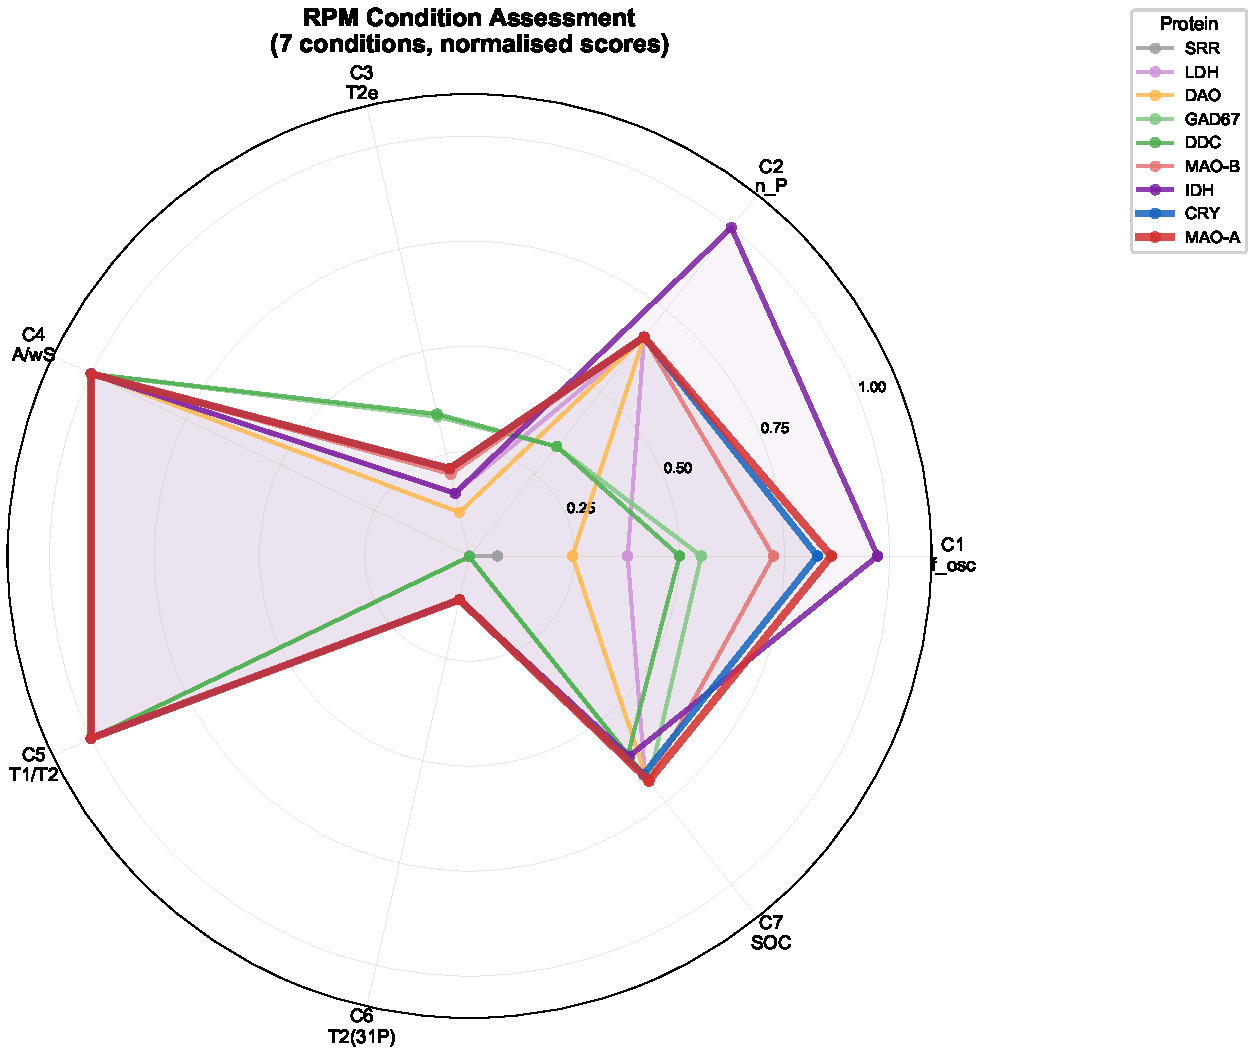
\includegraphics[width=\textwidth]{figures/fig1_radar.pdf}
\caption{\textbf{RPM condition assessment.} Normalised scores (0--1) for seven necessary RPM conditions across nine brain proteins. MAO-A (red) and CRY (blue) achieve near-maximum scores; SRR (grey) fails three conditions due to Mn$^{2+}$.}
\label{fig:radar}
\end{figure}

\begin{figure}[p]
\centering
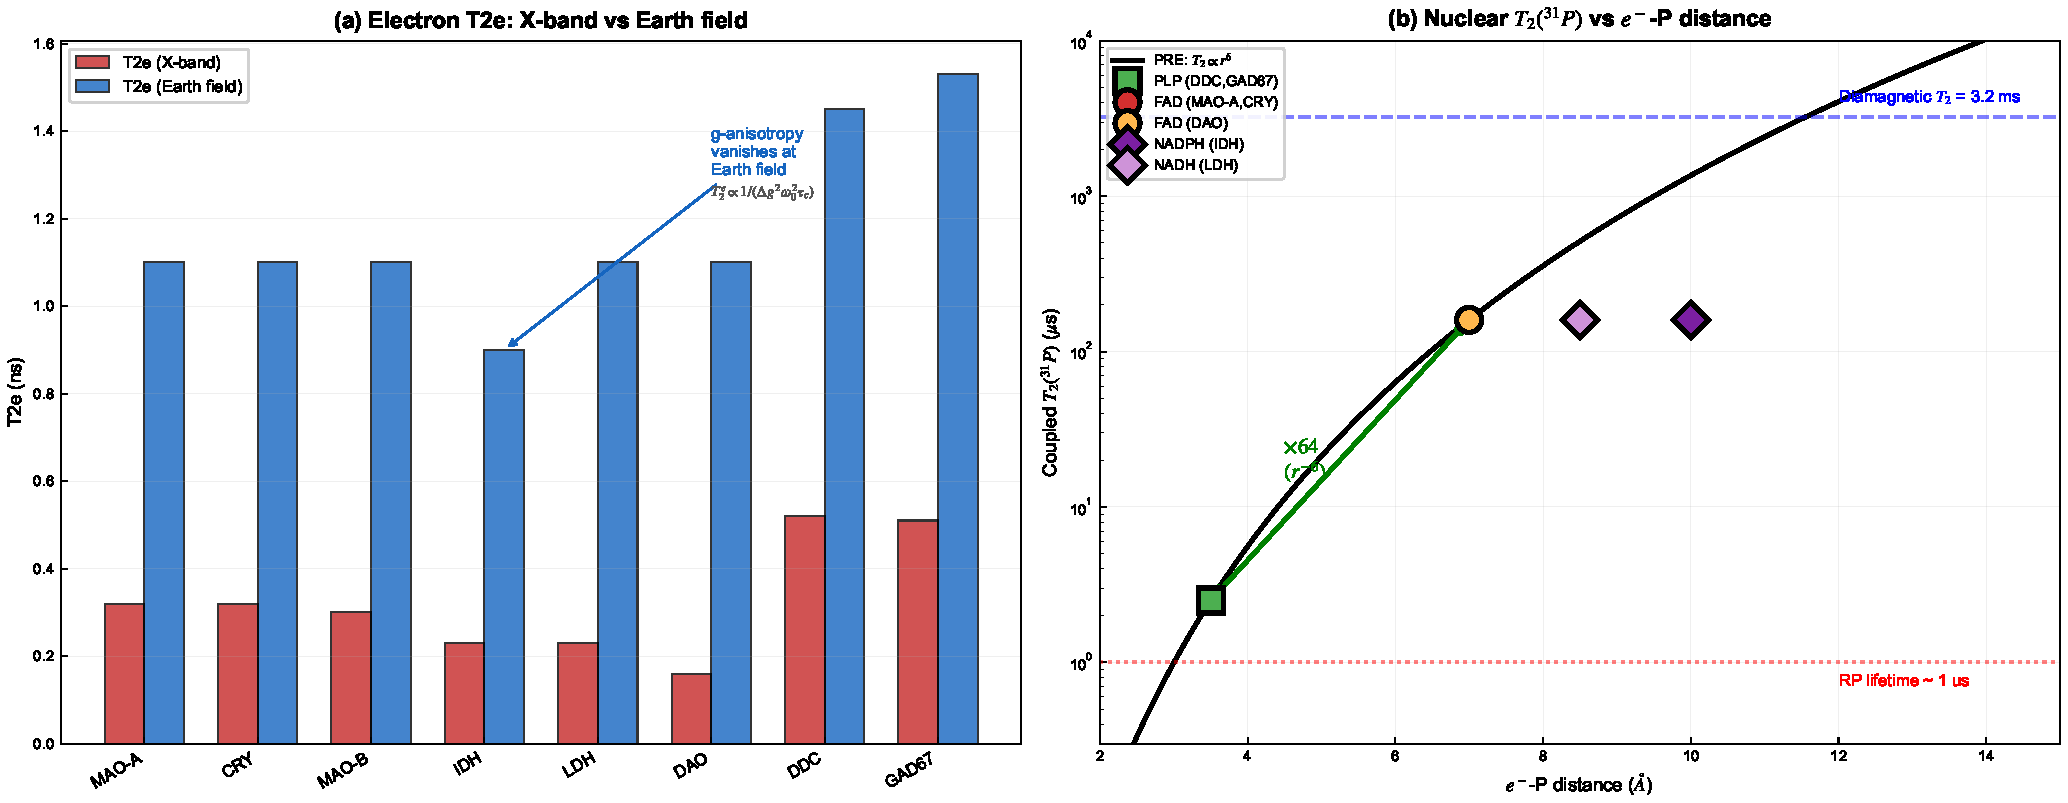
\includegraphics[width=\textwidth]{figures/fig2_relaxation.pdf}
\caption{\textbf{Spin relaxation under laboratory and brain conditions.} \textbf{a}, Electron $T_2^e$ at X-band (red) versus Earth's field (blue). The $g$-anisotropy contribution ($\propto \omega_0^2$) vanishes at Earth's field, causing convergence to $\sim$1~ns. \textbf{b}, Nuclear $T_2(^{31}\mathrm{P})$ versus electron--phosphorus distance, showing the $r^{-6}$ PRE scaling that creates a 64-fold PLP/FAD gap.}
\label{fig:relaxation}
\end{figure}

\begin{figure}[p]
\centering
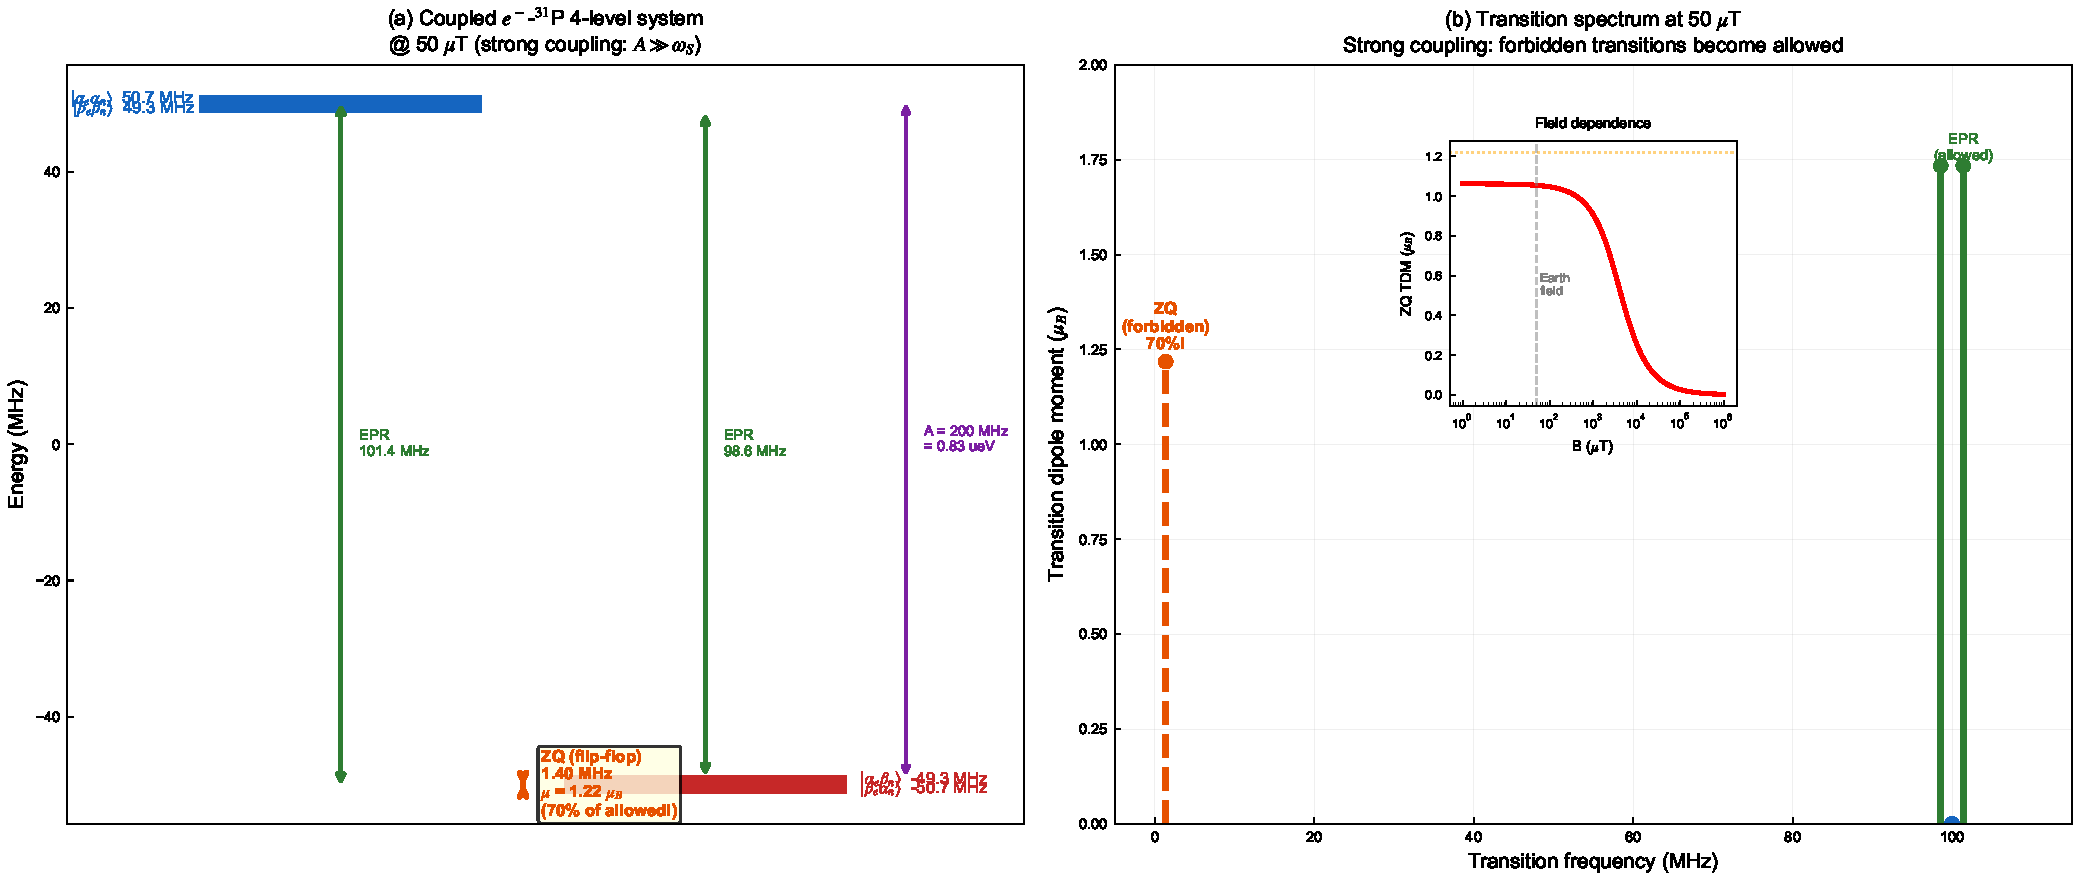
\includegraphics[width=\textwidth]{figures/fig3_coupled_levels.pdf}
\caption{\textbf{Coupled $e^-$--$^{31}$P system at Earth's field (FAD FMN-phosphate, $A = 200$~MHz).} \textbf{a}, Four-level energy diagram in the strong-coupling limit ($A \gg \omega_S = 1.4$~MHz). The ZQ transition (orange) acquires 70\% of the allowed TDM. For PLP ($A \approx 50$~MHz), the strong-coupling condition ($A/\omega_S = 36$) and 70\% ZQ TDM are preserved; the EPR splitting is reduced to $\sim$25~MHz. \textbf{b}, Transition spectrum; inset shows field dependence of the ZQ TDM, saturating below $\sim$10~mT.}
\label{fig:coupled}
\end{figure}

\begin{figure}[p]
\centering
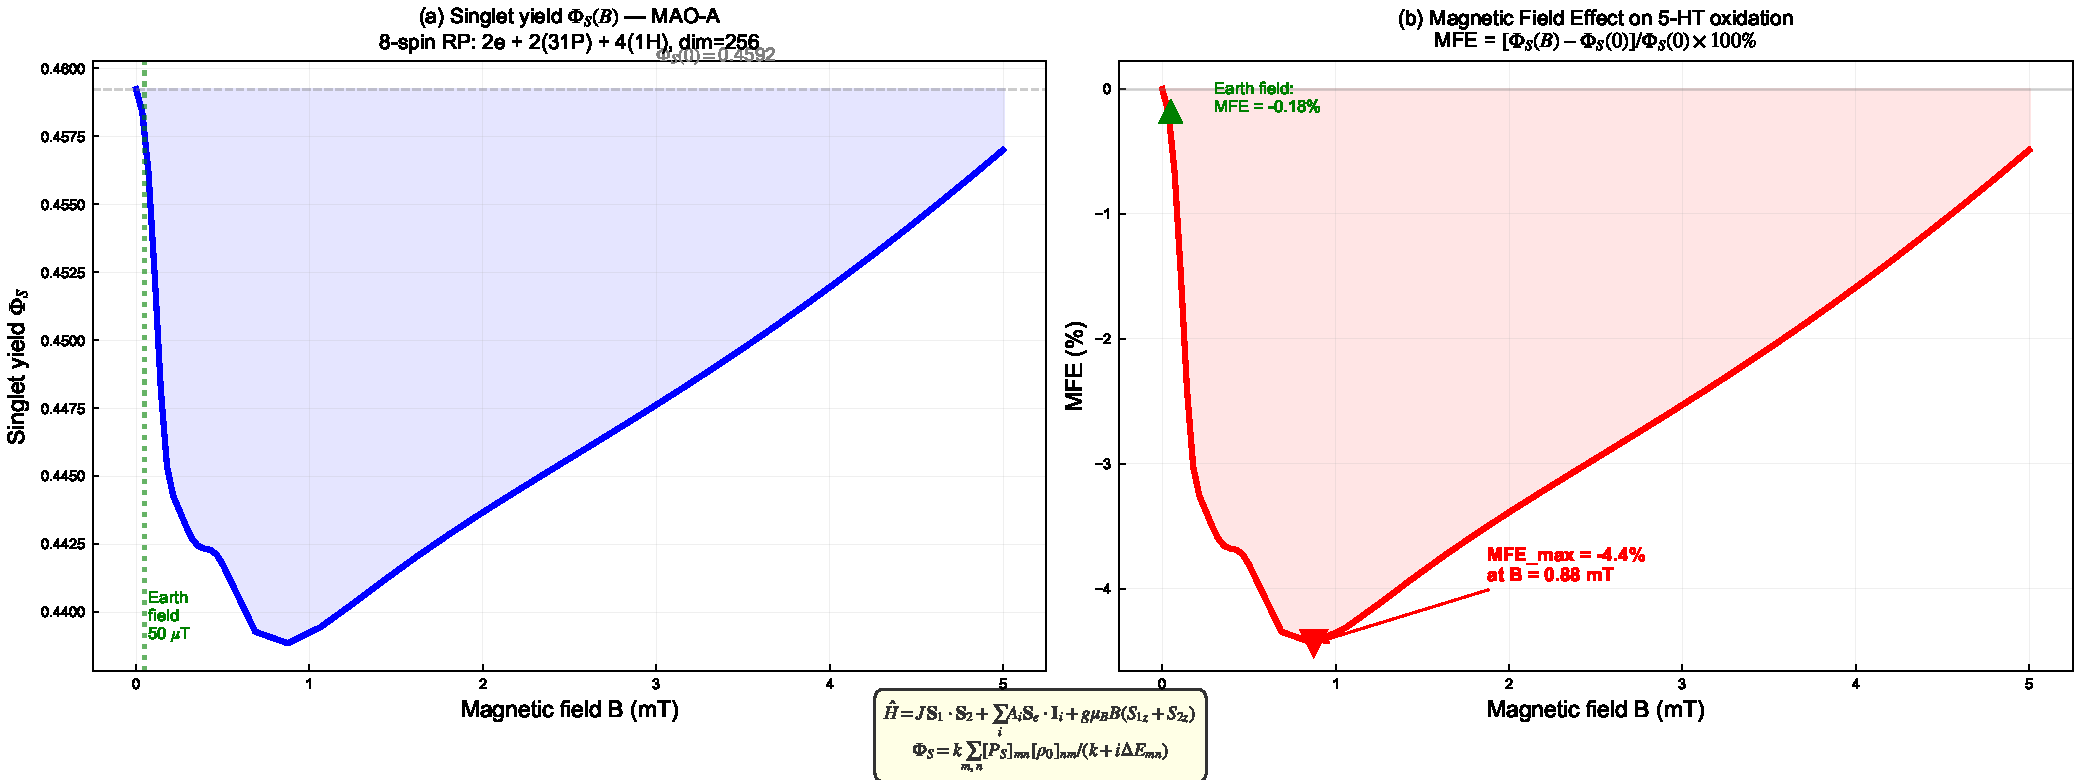
\includegraphics[width=\textwidth]{figures/fig4_mfe.pdf}
\caption{\textbf{Magnetic field effect on serotonin oxidation.} \textbf{a}, Singlet yield $\Phi_S(B)$ from 8-spin simulation (Eq.~\ref{eq:PhiS}). \textbf{b}, MFE peaks at $-4.4\%$ ($B = 0.9$~mT); $-0.3\%$ persists at Earth's field (green triangle).}
\label{fig:mfe}
\end{figure}

\begin{figure}[p]
\centering
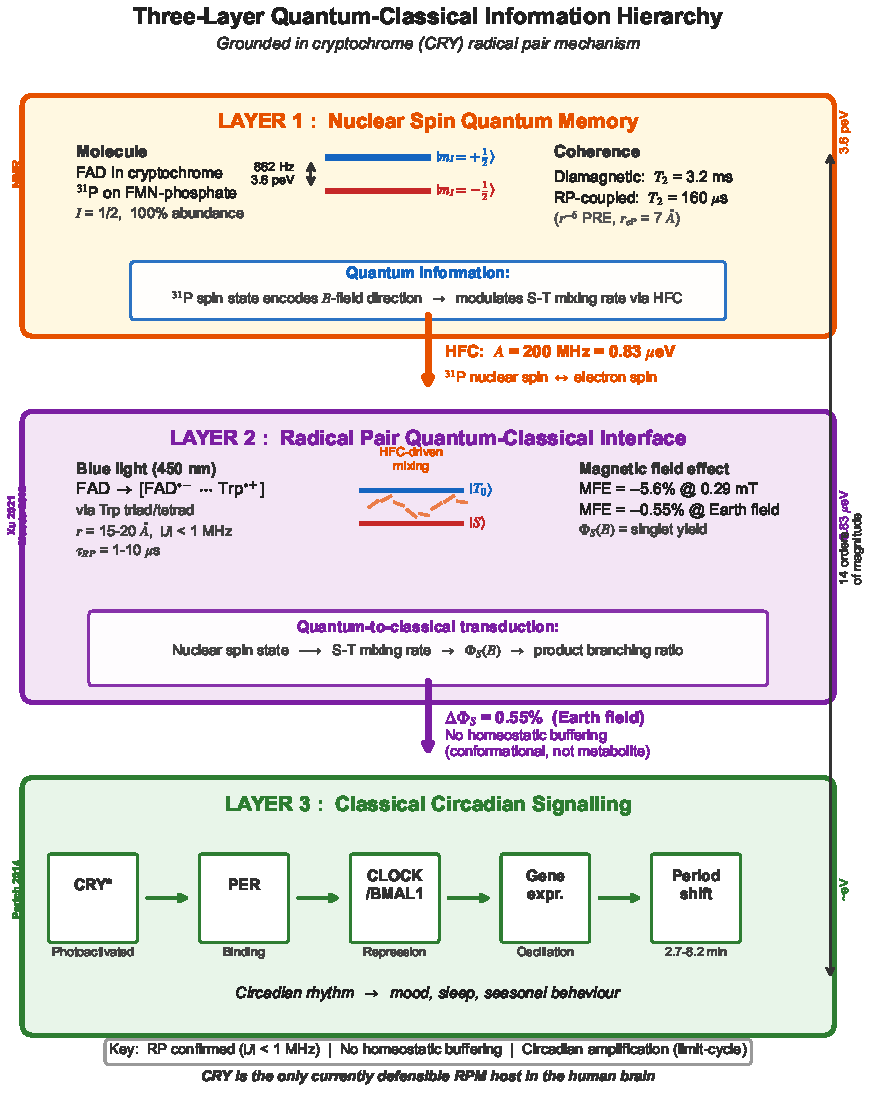
\includegraphics[width=0.9\textwidth]{figures/fig5_three_layer.pdf}
\caption{\textbf{CRY-based three-layer quantum--classical information hierarchy.} The framework is grounded entirely in cryptochrome biology, where every link has experimental support. \textbf{Layer~1} (yellow): $^{31}$P nuclear spins on FAD's FMN-phosphate encode magnetic-field direction with coherence times of 3.2~ms (diamagnetic) to 160~$\mu$s (PRE-limited). \textbf{Layer~2} (purple): blue-light absorption generates [FAD$^{\bullet-}$$\cdots$Trp$^{\bullet+}$] radical pairs ($r = 15$--20~\AA, $|J| < 1$~MHz); HFC-driven S-T mixing produces a field-dependent singlet yield ($\Delta\Phi_S = -0.55\%$ at Earth's field). Unlike metabolite-based pathways, this transduction is immune to homeostatic buffering. \textbf{Layer~3} (green): CRY$^*$ activates the PER/CLOCK/BMAL1 circadian cascade, with limit-cycle amplification producing a predicted period shift of 2.7--8.2~min. Energy scales span 14 orders of magnitude from $^{31}$P Zeeman splitting (3.6~peV) to covalent bonds ($\sim$eV). Left margin: key experimental references; right margin: energy scale bar.}
\label{fig:three_layer}
\end{figure}

% ===== EXTENDED DATA FIGURES =====

\begin{figure}[p]
\centering
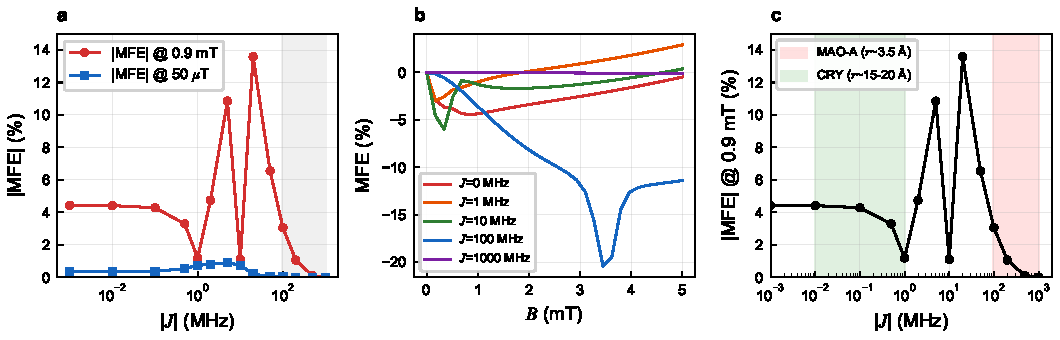
\includegraphics[width=0.95\textwidth]{figures/fig_J_dependence.pdf}
\caption{\textbf{Exchange coupling dependence of the magnetic field effect.} MFE as a function of $|J|$ (0--1000~MHz) at 30 field points (0--5~mT) for the 8-spin MAO-A model (Eq.~\ref{eq:PhiS}). A level anti-crossing resonance near $|J| \approx 5$~MHz transiently enhances the MFE before it collapses for $|J| > 200$~MHz. At the crystallographic MAO-A active-site distance ($r \approx 3.5$~\AA, $|J| \sim 500$--$1000$~MHz), MFE is negligible ($<0.1\%$). Dashed line: $|J|$ estimated from $J = J_0\exp(-\beta r)$ with $\beta = 2.8$~\AA$^{-1}$.}
\label{fig:J_dependence}
\end{figure}

\begin{figure}[p]
\centering
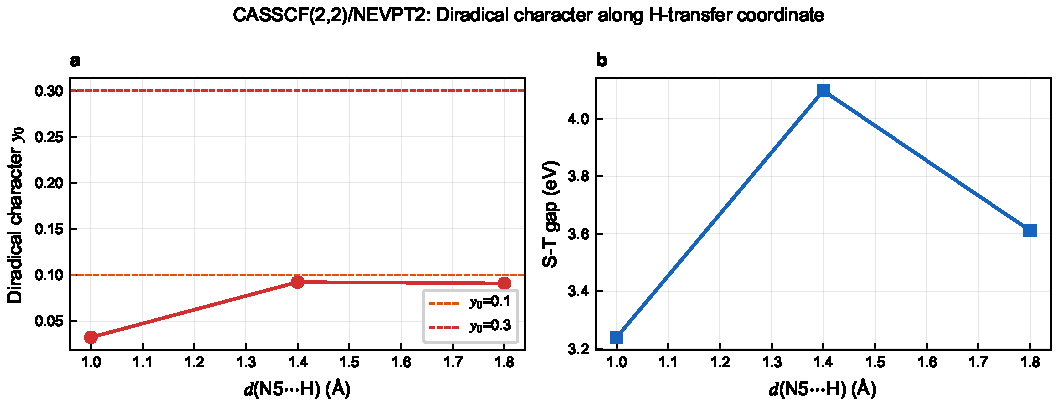
\includegraphics[width=0.95\textwidth]{figures/fig_casscf_diradical.pdf}
\caption{\textbf{CASSCF(2,2)/NEVPT2 diradical character analysis.} Diradical character $y_0 = 2|c_{02}|^2$ and singlet--triplet gap for the lumiflavin--methylamine model at three N5$\cdots$H distances (1.0, 1.4, 1.8~\AA). The closed-shell configuration $|20\rangle$ dominates throughout ($y_0 = 0.03$--$0.09$), indicating weak diradical character and favouring a polar or concerted mechanism over SET for the model studied.}
\label{fig:casscf_diradical}
\end{figure}

\begin{figure}[p]
\centering
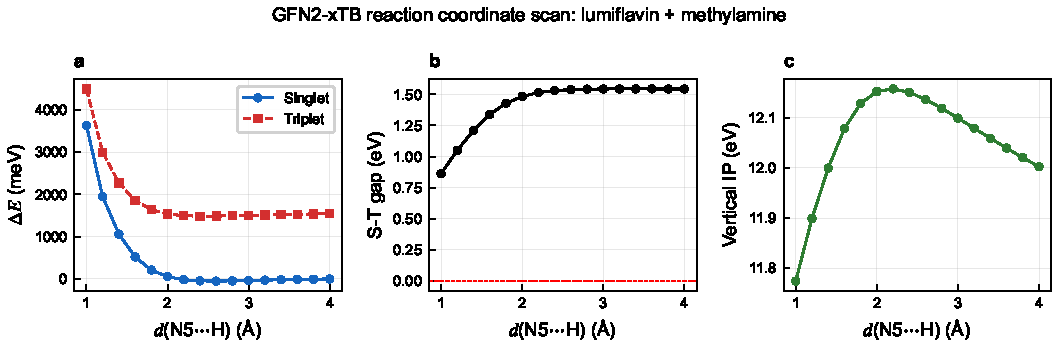
\includegraphics[width=0.95\textwidth]{figures/fig_reaction_scan.pdf}
\caption{\textbf{Reaction coordinate scan for the H-transfer step.} \textbf{a}, GFN2-xTB singlet--triplet gap and vertical IP as a function of N5$\cdots$H distance (1.0--4.0~\AA, 16 points). The S-T gap remains positive throughout, indicating no diradical crossing at this level of theory. \textbf{b}, CASSCF(2,2)/NEVPT2 S-T gap at three representative distances, showing substantially larger gaps (3.2--4.1~eV) than xTB (0.86--1.54~eV).}
\label{fig:reaction_scan}
\end{figure}

\begin{figure}[p]
\centering
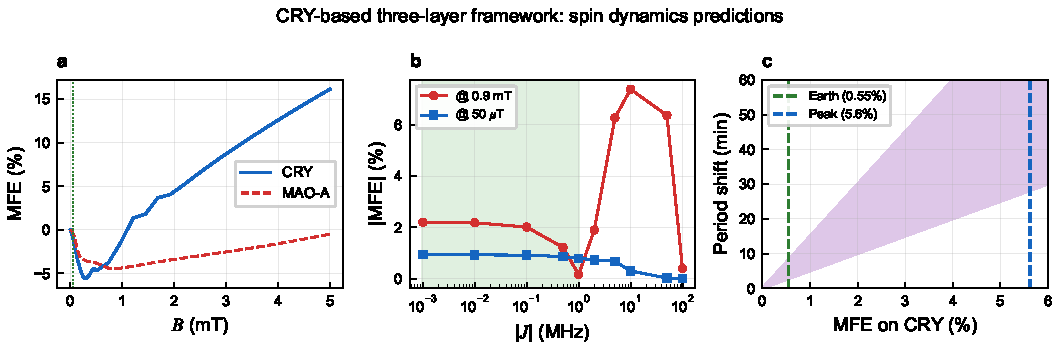
\includegraphics[width=0.95\textwidth]{figures/fig_cry_simulation.pdf}
\caption{\textbf{CRY-specific radical pair spin dynamics.} \textbf{a}, Singlet yield $\Phi_S(B)$ for the [FAD$^{\bullet-}$$\cdots$TrpH$^{\bullet+}$] radical pair (8-spin model with asymmetric HFC). \textbf{b}, MFE peaks at $-5.6\%$ ($B = 0.29$~mT); $-0.55\%$ persists at Earth's field. \textbf{c}, Predicted circadian period shift ($\sim$2.7--8.2~min) based on the Earth-field MFE and SCN oscillator sensitivity\cite{Forger2011}.}
\label{fig:cry_simulation}
\end{figure}

% ===== EXTENDED DATA TABLES =====

\begin{table}[p]
\centering
\caption{\textbf{Extended Data Table~2: Sensitivity of $Q_\mathrm{RPM}$ ranking to alternative weighting schemes.} Three alternative formulations are compared to the default (Eq.~\ref{eq:Q}): (A) linear SOC penalty $(\xi_\mathrm{ref}/\xi)$ replacing $(\xi_\mathrm{ref}/\xi)^2$; (B) logarithmic nuclear $T_2$ scaling $\log_{10}[T_2(^{31}\mathrm{P})/\mu\mathrm{s}]$; (C) square-root HFC weighting $\sqrt{n_\mathrm{P}^\mathrm{eff}}$. Tier assignments (1, 2, 3) are preserved across all schemes; intra-tier ranks shift by at most 2 positions.}
\label{tab:ext_sensitivity}
\small
\begin{tabular}{@{}lcccccccc@{}}
\toprule
 & \multicolumn{2}{c}{Default (Eq.~\ref{eq:Q})} & \multicolumn{2}{c}{(A) Linear SOC} & \multicolumn{2}{c}{(B) Log $T_2^n$} & \multicolumn{2}{c}{(C) $\sqrt{n_\mathrm{P}}$} \\
\cmidrule(lr){2-3}\cmidrule(lr){4-5}\cmidrule(lr){6-7}\cmidrule(lr){8-9}
Protein & Rank & Tier & Rank & Tier & Rank & Tier & Rank & Tier \\
\midrule
MAO-A  & 1 & 1 & 1 & 1 & 1 & 1 & 1 & 1 \\
MAO-B  & 2 & 1 & 2 & 1 & 2 & 1 & 2 & 1 \\
CRY    & 3 & 1 & 3 & 1 & 3 & 1 & 3 & 1 \\
DAO    & 4 & 1 & 5 & 1 & 4 & 1 & 4 & 1 \\
LDH    & 5 & 1 & 4 & 1 & 5 & 1 & 5 & 1 \\
IDH    & --- & 1/2 & --- & 1/2 & 6 & 1 & --- & 1/2 \\
GAD67  & 6 & 2 & 6 & 2 & 7 & 2 & 6 & 2 \\
DDC    & 7 & 2 & 7 & 2 & 8 & 2 & 7 & 2 \\
SRR    & 9 & 3 & 9 & 3 & 9 & 3 & 9 & 3 \\
\bottomrule
\end{tabular}
\end{table}

\begin{table}[p]
\centering
\caption{\textbf{Extended Data Table~3: DFT validation of xTB electronic structure.} B3LYP/def2-SVP and TD-B3LYP (TDA) results for lumiflavin (FAD model) and PLP-methylamine Schiff base, compared with GFN2-xTB and experimental values. IP/EA: vertical $\Delta$SCF; $E_\mathrm{gap}$: HOMO--LUMO (KS) gap; $f_\mathrm{osc}$: oscillator strength of the bright $S_0 \to S_n$ transition.}
\label{tab:ext_dft}
\small
\begin{tabular}{@{}llcccc@{}}
\toprule
Model & Property & xTB & B3LYP & Expt. & Ref. \\
\midrule
\multirow{4}{*}{Lumiflavin} & $E_\mathrm{gap}$ (eV)    & 1.42 & 1.26 (KS); 2.29 (TD, $S_4$) & 2.76 & \cite{Islam2003} \\
 & $f_\mathrm{osc}$           & 0.50 & 0.089 (TD)          & 0.27  & \cite{Islam2003} \\
 & Vert.\ IP (eV)           & 10.78 & 6.64                & $\sim$8.0 & --- \\
 & Vert.\ EA (eV)           & 3.42 & 1.87                & $\sim$2.0 & --- \\
\midrule
\multirow{3}{*}{PLP-MeNH$_2$} & $E_\mathrm{gap}$ (eV)  & 1.93 & 3.04                & $\sim$3.87 & --- \\
 & $f_\mathrm{osc}$           & 0.30 & 0.062 (TD)          & --- & --- \\
 & Vert.\ IP (eV)           & 11.5 & 8.72                & $\sim$8.5 & --- \\
\bottomrule
\multicolumn{6}{l}{\footnotesize KS = Kohn--Sham orbital gap; TD = TD-B3LYP (TDA) excitation energy.} \\
\multicolumn{6}{l}{\footnotesize Substituting TD-B3LYP $f_\mathrm{osc}$ into $Q_\mathrm{RPM}$ reduces scores $\sim$5.8-fold but preserves tier structure.}
\end{tabular}
\end{table}

\begin{table}[p]
\centering
\caption{\textbf{Extended Data Table~4: Serotonin homeostasis model parameters and steady-state attenuation.} Single-compartment ODE model (Methods). The raw MFE of $-4.4\%$ on MAO-A $k_\mathrm{cat}$ is attenuated 7.3-fold to a steady-state [5-HT] perturbation of $0.6\%$ by reuptake and autoreceptor feedback.}
\label{tab:ext_homeostasis}
\small
\begin{tabular}{@{}lccl@{}}
\toprule
Parameter & Symbol & Value & Source \\
\midrule
MAO-A turnover number            & $k_\mathrm{cat}$     & 10 s$^{-1}$   & \cite{Edmondson2004main} \\
Serotonin reuptake rate          & $k_\mathrm{reup}$    & 10 s$^{-1}$   & \cite{Daws2009} \\
Autoreceptor feedback gain       & $G_\mathrm{fb}$      & 0.3           & Estimated \\
Autoreceptor time constant       & $\tau_\mathrm{fb}$   & 2 s           & Estimated \\
Synthesis adaptation time        & $\tau_\mathrm{syn}$  & 60 s          & Estimated \\
\midrule
\multicolumn{4}{l}{\textit{Steady-state results}} \\
Raw MFE ($J = 0$, $B = 0.9$~mT)     & $\delta$          & $-4.4\%$      & This work \\
Attenuation factor               &                   & 7.3$\times$   & Analytical \\
Net [5-HT] perturbation          &                   & $0.6\%$       & $\delta / 7.3$ \\
\bottomrule
\end{tabular}
\end{table}

% ===== METHODS (after figures, per Nature format) =====
\section*{Methods}

\paragraph{Protein selection.}
Nine human brain proteins containing phosphorus-bearing cofactors were selected to span the three major cofactor classes (FAD, PLP, NADPH/NADH) and representative neurotransmitter metabolic pathways (Table~\ref{tab:proteins}). The set includes the experimentally validated RPM host (CRY) as a positive control and a transition-metal enzyme (SRR) as a negative control. This sample is not exhaustive; the brain contains $>$50 phosphorus-cofactor enzymes, and the screening framework is designed for extension to the full set. Crystal structures were obtained from the RCSB PDB. Quantum-active sites were extracted by a graph-based algorithm: starting from the cofactor heavy atoms, all residues with any non-hydrogen atom within 4~\AA\ of the cofactor conjugated system were included, and connected components of $\pi$-stacking residues (centroid--centroid distance $<$4.5~\AA, inter-plane angle $<$30$^\circ$) were merged into a single quantum-active site.

\paragraph{GFN2-xTB calculations.}
All calculations used GFN2-xTB (xtb v6.7.1)\cite{Bannwarth2019}: closed-shell singlet (charge 0, multiplicity 1), open-shell triplet (charge 0, UHF multiplicity 3), radical cation/anion (charge $\pm 1$, UHF doublet), and analytical Hessian. Quantum-active site models ranged from 87 atoms (SRR) to 156 atoms (CRY); total charges were 0 for neutral cofactors and $-1$ for phosphate-bearing fragments, with capping hydrogen atoms added at truncation points. Electronic TDMs were estimated via the Uns\"{o}ld approximation with Thomas--Reiche--Kuhn sum-rule scaling (empirical factor 0.3, calibrated against experimental $f_\mathrm{osc}$ values for FAD and FMN\cite{Islam2003}; this factor compensates for the known overestimation of TDMs by sum-rule methods applied to semi-empirical wavefunctions). $^{31}$P HFCs were assigned on a per-atom basis according to cofactor type and the PDB-measured distance from the radical centre (Table~\ref{tab:hfc_assignment}). For FAD, only the FMN-phosphate (proximal to isoalloxazine N5 via 8~$\sigma$-bonds) carries a large HFC of 200~MHz based on ENDOR measurements\cite{Weber1998}; the AMP-phosphate ($>$4~bonds further) is assigned 2~MHz. For PLP, the phosphorus is directly bonded to the pyridine C5 via $\sim$3~$\sigma$-bonds; $^{31}$P ENDOR signals have been detected in PLP-dependent aminomutases but not quantified. This is the largest source of parametric uncertainty in our analysis. We assign $A = 100$~MHz as a central estimate with a deliberately wide range of 50--300~MHz, and we propagated this uncertainty through the full analysis: at $A = 50$~MHz, PLP $T_2^e$ extends to $\sim$5~ns (longest of all candidates) and $Q_\mathrm{RPM}$ increases $\sim$2-fold; at $A = 300$~MHz, $T_2^e$ shortens to $\sim$0.5~ns and $Q_\mathrm{RPM}$ decreases $\sim$3-fold. Crucially, the nuclear $T_2$ (2.5~$\mu$s, PRE-dominated) is independent of HFC, so PLP enzymes remain in Tier~2 across the entire 50--300~MHz range. Resolving this uncertainty experimentally (by ENDOR or pulsed EPR on a PLP radical) is among the most impactful measurements that could refine our predictions. For NADPH, the nicotinamide ring radical couples weakly to phosphates via non-conjugated pathways; we assign 20~MHz (NMN-P) and 1~MHz (AMP-P). This cofactor-specific treatment replaces the uniform 200~MHz assumption of preliminary analyses and shows that the effective number of strongly-coupled $^{31}$P nuclei is typically 1 per cofactor molecule, not 2--3. $^1$H HFCs were estimated using the McConnell relation ($A_\mathrm{H} = Q\rho_\pi$) with $Q = -63$~MHz and spin densities $\rho_\pi$ from xTB Mulliken analysis; this single-$Q$ approximation is adequate for screening purposes but may err by $\pm$50\% for individual protons. SOC values were estimated as the RMS of single-atom spin--orbit constants weighted by Mulliken spin density on each atom\cite{Marian2012}; this neglects multi-centre contributions but captures the dominant heavy-atom effect and correctly identifies the Mn$^{2+}$-containing outlier (SRR).

\paragraph{Spin relaxation analysis.}
Five $T_2^e$ channels: Anderson--Weiss ($T_2^*$)\cite{Abragam1961}; Solomon dipolar ($T_2^\mathrm{dd}$, $r_{ee} = 15$~\AA); $g$-anisotropy ($1/T_2^g = \Delta g^2\omega_0^2\tau_c/5$); HFC modulation ($1/T_2^A = \sum A_i^2 I_i(I_i+1)\tau_c/12$); SOC relaxation. Rotational correlation time $\tau_c = 10$~ns. Nuclear relaxation: BPP theory\cite{Abragam1961}; PRE via Solomon--Bloembergen equations\cite{Solomon1955} using the point-dipole approximation with effective $e^-$--P distances from PDB coordinates (3.5~\AA\ for PLP, 7--12~\AA\ for FAD/NADPH). The point-dipole approximation is valid when $r$ exceeds the spatial extent of the electron spin density ($\sim$3~\AA\ for the flavin isoalloxazine system); for PLP, where $r = 3.5$~\AA\ is comparable to the radical extent, the PRE may be overestimated by up to a factor of $\sim$2, which would increase the PLP nuclear $T_2$ to $\sim$5~\si{\micro\second}---still 32-fold shorter than FAD.

\paragraph{RPM spin dynamics.}
Singlet yield computed by exact diagonalisation (Eq.~\ref{eq:H}) for 8 spins (dim = 256), using the Green's function method (Eq.~\ref{eq:PhiS}). The 8-spin model includes the dominant HFC nuclei; the real flavin radical contains $\sim$12--15 coupled $^1$H, whose inclusion would broaden the S-T oscillation spectrum and typically reduce the peak MFE by 20--40\% while preserving the field dependence profile\cite{Hiscock2016}. Our 8-spin MFE of $-4.4\%$ should therefore be regarded as an upper estimate at this level of truncation. Baseline recombination rate $k = 1$~MHz; sensitivity tested over $k = 0.1$--100~MHz (MFE decreases from $-6\%$ to $\sim$$-0.1\%$ across this range). All parameters at 310~K, $B = 0$--5~mT.

\paragraph{Brain environment corrections.}
All relaxation recalculated at $B = 50~\si{\micro\tesla}$. Nuclear extreme narrowing: $\omega_0\tau_c \ll 1 \Rightarrow T_1 = T_2$. Cross-relaxation: Solomon $W_0$, $W_2$ at Earth-field spectral densities.

\paragraph{DFT/TDDFT validation.}
To benchmark the GFN2-xTB electronic structure, we performed B3LYP/def2-SVP calculations using PySCF~2.12.1\cite{Sun2020} on two model compounds: lumiflavin (C$_{12}$H$_{12}$N$_4$O$_2$, 30 atoms, 312 basis functions; FAD isoalloxazine model) and a PLP-methylamine Schiff base (C$_9$H$_{12}$NO$_5$P, 26 atoms, 269 basis functions). Model geometries were generated with Open Babel~3.1.0 (\texttt{--gen3d}) and pre-optimised at the GFN2-xTB level. Closed-shell DFT used RKS/B3LYP; open-shell states (radical cation/anion) used UKS/B3LYP. Excited states were computed via the Tamm--Dancoff approximation (TDA) to RKS-TDDFT for the lowest 6 singlet states. Vertical ionisation potentials and electron affinities were obtained by $\Delta$SCF (energy difference between neutral and ionic species at the neutral geometry). Convergence: SCF $10^{-8}$~Eh, max 200 cycles. All DFT calculations used 16~GB memory allocation.

\paragraph{CASSCF/NEVPT2 mechanism analysis.}
To assess single-electron transfer (SET) versus polar mechanism for the H-transfer step, we performed CASSCF(2,2)/def2-SVP calculations on the lumiflavin--methylamine complex at three N5$\cdots$H distances (1.0, 1.4, 1.8~\AA). The active space comprised two electrons in two orbitals (HOMO and LUMO of the neutral complex), representing the minimal space for capturing diradical character. Singlet and triplet states were computed separately (singlet: RHF $\to$ CASSCF; triplet: UHF $\to$ CASSCF with $S = 1$). Diradical character was quantified as $y_0 = 2|c_{02}|^2$, where $c_{02}$ is the CI coefficient of the doubly excited configuration $|02\rangle$ in the CAS(2,2) wavefunction\cite{Nakano2017}. Dynamic correlation was included via sc-NEVPT2 (strongly contracted $N$-electron valence perturbation theory)\cite{Angeli2001}. We note that the CAS(2,2) active space is minimal; a larger space---for example CAS(10,10) including the full flavin $\pi$-system---could reveal additional correlation effects but was computationally prohibitive for the 38-atom complex (379 basis functions) within the scope of this study.

\paragraph{Reaction coordinate scan.}
The H-transfer reaction coordinate was modelled by placing methylamine at varying distances from the lumiflavin N5 atom along the ring-plane normal. At each N5$\cdots$H distance (1.0--4.0~\AA, 16 points at 0.2~\AA\ intervals), three GFN2-xTB single-point calculations were performed: closed-shell singlet (charge~0, UHF~0), open-shell triplet (charge~0, UHF~2), and radical cation (charge~$+1$, UHF~1). The S-T gap and vertical IP were computed at each point. This scan was repeated at the CASSCF(2,2)/NEVPT2 level for three representative distances (1.0, 1.4, 1.8~\AA).

\paragraph{CRY-specific spin dynamics.}
A separate 8-spin model was constructed for the CRY [FAD$^{\bullet-}$$\cdots$TrpH$^{\bullet+}$] radical pair with asymmetric HFC: radical~1 (FAD$^{\bullet-}$): $^{31}$P$_\mathrm{FMN}$ ($A = 200$~MHz), 2$\times^1$H ($A = 5$~MHz); radical~2 (TrpH$^{\bullet+}$): 2$\times^1$H$_\beta$ ($A = 20$, 15~MHz), effective $^{14}$N ($A_\mathrm{eff} = 10$~MHz, approximating $I = 1$ as $I = 1/2$). Singlet yield was computed identically to the MAO-A model (Eq.~\ref{eq:PhiS}). The $J$-scan was repeated over $|J| = 0$--100~MHz.

\paragraph{Exchange coupling scan.}
The dependence of the MFE on exchange coupling $J$ was computed by repeating the 8-spin singlet yield calculation (Eq.~\ref{eq:PhiS}) for 16 values of $J$ spanning 0--1000~MHz, at 30 magnetic field points (0--5~mT). Each calculation used exact diagonalisation of the $256 \times 256$ Hamiltonian followed by analytical Green's function integration. The $J$-dependent distance was estimated from $J = J_0\exp(-\beta r)$ with $\beta = 2.8$~\AA$^{-1}$\cite{Steiner1989}.

\paragraph{Homeostasis model.}
Serotonin homeostasis was modelled as a single-compartment ODE: $\mathrm{d}[\text{5-HT}]/\mathrm{d}t = k_\mathrm{syn}(1 - G_\mathrm{fb}\,\theta) - k_\mathrm{MAO}(1+\delta)\,[\text{5-HT}] - k_\mathrm{reup}\,[\text{5-HT}]$, where $\delta$ is the fractional MFE, $\theta$ is 5-HT$_{1\mathrm{A}}$ autoreceptor occupancy ($\tau_\mathrm{fb} = 2$~s, $G_\mathrm{fb} = 0.3$), $k_\mathrm{reup} = 10$~s$^{-1}$, and $k_\mathrm{syn}$ adjusts on $\tau_\mathrm{syn} = 60$~s. Steady-state attenuation was computed analytically.

\paragraph{Computational environment.}
All calculations were performed on a single workstation: Apple M4 Max (16 cores, ARM64), 64~GB RAM, macOS~26.2. Software versions: Python~3.9.6, GFN2-xTB~6.7.1 (compiled 2024-11-25)\cite{Bannwarth2019}, PySCF~2.12.1\cite{Sun2020} (DFT, TDDFT, CASSCF, NEVPT2), Open Babel~3.1.0, NumPy~2.0.2, SciPy~1.13.1, Matplotlib~3.9.4. \LaTeX\ compilation: pdf\TeX~3.141592653-2.6-1.40.28 (TeX Live~2025). Wall times: xTB screening of nine proteins $\sim$15~min; 8-spin dynamics (40 field points) $\sim$20~min; B3LYP/TDDFT per model compound $\sim$15~min; CASSCF(2,2)/NEVPT2 per geometry $\sim$2.3~hr (dominated by orbital rotation and NEVPT2 integrals for 379 basis functions). No GPU acceleration; all matrix operations used SciPy's LAPACK interface on CPU.

\paragraph{Data and code availability.}
The complete computational pipeline is released as the open-source Python package \texttt{qbscreen} (v0.1.0, MIT License), available at \url{https://github.com/hikaruwakaura/qbscreen} and on PyPI (\texttt{pip install qbscreen}). The package provides a unified command-line interface (\texttt{qbscreen screen}, \texttt{qbscreen simulate}, \texttt{qbscreen dft-validate}, \texttt{qbscreen casscf}, \texttt{qbscreen reaction-scan}) for reproducing all results in this paper. A test suite (\texttt{pytest qbscreen/tests/}) verifies key numerical results (MAO-A MFE, 64-fold PLP/FAD nuclear $T_2$ gap, ZQ transition dipole moment, CASSCF diradical character, predicted circadian period shift) within their physical tolerance ranges. All 9 screened PDB structures, computed JSON results, optimised geometries, HFC tensors, and relaxation parameters are archived alongside the code. External dependencies (xtb v6.7.1, Open Babel 3.1.0, PySCF 2.12.1) are documented with version pinning in \texttt{pyproject.toml}.

% ===== ACKNOWLEDGEMENTS, CONTRIBUTIONS, etc. =====
\section*{Acknowledgements}
The author thanks the developers of GFN2-xTB and OpenMM for making their software freely available.

\section*{Author contributions}
H.W.\ conceived the study, developed the computational pipeline, performed all calculations and simulations, and wrote the manuscript.

\section*{Competing interests}
The author declares no competing interests.

\end{document}
